The Multi-Band Template Analysis (MBTA) is one of the search pipelines running on the LIGO and Virgo data streams.
It uses the matched filtering technique to search for CBC signals, both online at low-latency and offline.
This technique, detailled in section \ref{sec:matched_filter}, consists in computing the cross-correlation of the data with templates which are predictions of the signal being searched for.
The result of this operation, called also filtering, is the Signal-to-Noise Rartio (SNR) time series, which becomes large at the time of an event. 
Since we don't know the parameters of the source, this operation is performed on multiple templates, the template bank.
The goal is to find the template which maximizes the SNR in order the find the source parameters and get a candidate, or trigger, if the SNR is above a given threshold.

MBTA filters the data at a low computational cost by splitting the filtering in two separate frequency bands.
This splitting has two benefits.
First, it allows a tuning of the sampling frequency differently and template duration for each band, effectively reducing the time needed to compute the Fast Fourier Transforms (FFT) needed for the filtering.
Second, it significantly reduces the number of templates needed to cover the parameter space.
The result of the matched-filtering in each band is then coherently combined yielding the time series for the full frequency band.
But a search pipeline is not just the matched filtering. There are preprocessing steps as well as post processing, to clean the data and evaluate the quality of the candidates. This chapter describes all the steps of the MBTA pipeline.


%%%%%%%%%%
\subsection{Overview of the MBTA pipeline}
\label{sec:MBTA}
A schematic view of the pipeline is given in figure \ref{fig:mbta_scheme}.
We describe here the main search of the pipeline dedicated to BNS, BBH and NSBH detection.
The online version for more specific searches (sub-solar mass search and early-warning) and offline version follow the same logic, with a few changes for some parameters like the sampling rate of analysis.
% We describe here the online version of the pipeline.
%The offline version follows the same logic.

MBTA takes the data of the LIGO and Virgo detectors to search for CBC signals.
There are two pre-processing steps before MBTA analyzes the data: the data coming from LIGO and Virgo are resampled by MBTA from \SI{16384}{Hz} to \SI{4096}{Hz}.
Then MBTA applies what is called the gating.
The gating is a noise rejection tool which removes loud glitches (transient noises) from the time series.
The gating is described in more details in section \ref{sec:gating}.

The data are then broadcasted to the machines that will do the filtering.
The filtering is done in parallel with 43 jobs (job 90 is specific to very short templates, see section \ref{sec:bankO4}) plus an additional one without gating (named region 4 or R4, see section \ref{sec:gating}).
Each of these jobs analyzes the data with a fraction of the template bank (and therefore a fraction of the parameter space) sorted by template duration.
This sorting allows to share them among jobs in such a way that most real templates are used by only one job.
Jobs which filter using long templates are given less templates to balance their computing usage.

The filtering is done using MBTA's own template banks.
The templates used for the matched-filtering are derived from accurate models of general relativity.
The template banks are built in order to have a loss of at most few percent in SNR (with respect to the optimal SNR) when detecting a signal.
They will be described in section \ref{sec:param_space}.

%The details of separation of the filtering in two bands are given in section \ref{sec:2bands}.
%More details on the PSD computation are given in section \ref{sec:psd_compute}.
If at some point the SNR is greater than a pre-defined threshold we say that we have a single detector trigger and the event will be saved.
During O3, the time of the trigger was taken as the time of the end of the template.
For O4 it is taken as the time of the maximum amplitude, the difference being the ringdown time.

The MBTA pipeline also uses data quality monitoring and a variety of noise rejection tools to either downgrade the SNR of triggers or straight off reject them to better discriminate astrophysical signals from background triggers.
Some are applied during the filtering and others at the post-filtering step.

The pipeline then searches for coincident triggers in different detectors, meaning observed with the same template and matching time accounting for the time of flight of gravitational waves between each pair of detectors.

An astrophysical signal or loud noise may match with several templates thus creating several triggers.
To avoid this redundancy, triggers that are neighbours in time are clustered (more on this in sections \ref{sec:single_search} and \ref{sec:clustering}).

The pipeline also computes a probability of astrophysical origin, a source classification and a False Alarm Rate (FAR) (see sections \ref{sec:far_coinc} and \ref{sec:pastro}).
Significant triggers are astrophysical candidates.
If their FAR is below a given threshold, they are uploaded to the Gravitational-Wave Candidate Event Database (GraCEDb) and online public alerts may be issued.


\begin{figure}
  \centering
  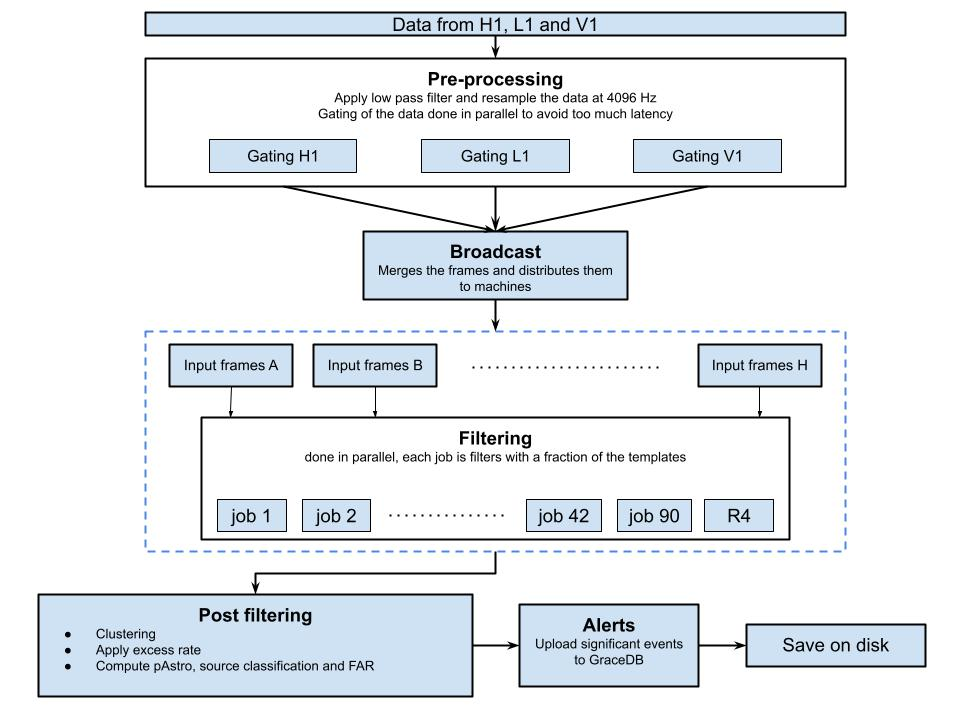
\includegraphics[width=0.65\linewidth]{sectionMBTA/schemaMBTA.jpg}
  \caption{Schematic of the processes and workflow of the online MBTA pipeline.}
  \label{fig:mbta_scheme}
\end{figure}




%%%%%%%%%%
\subsection{Gating}
\label{sec:gating}

Strain data sent to the pipeline are accompanied by a state vector.
This vector indicates whether the data can be safely analyzed.
Offline, this role is filled by the category 1 (CAT1) flags \cite{cat1_virgo,dq_flag} which indicate times at which major issues took place.
These times are not analyzed.

Yet, not all noisy periods are excluded by such vetoes.
For this reason, pipelines have to use a variety of noise rejection tools in order to control their background.
The gating is one of them.
We present here the gating as it was used during O3.
More details on the development of the gating can be found in \cite{aubin2020}.
The gating is a tool used to reject loud glitches.
It works by applying a gate function, hence the name, to set the $h(t)$ time series to 0.
Simply ignoring the data at the time where the glicth was identified is not enough because due to the finite size of the FFT, loud glicthes could spoil the full time series of one FFT.
It could therefore contaminate the data even after the glitch, it is thus mandatory to nullify the data.

Figure \ref{fig:strain_gated} shows the application of gating around a glitch in L1.
The gating process takes place before MBTA starts analyzing the data.
The criteria to apply the gating is based on the BNS range of the detector which follows the variations of the PSD of the detector.
If at some point the BNS range drops below 60\% of the median BNS range over the last 10 seconds, the gate function is applied.
This threshold is updated every second.
The range is computed for a BNS signal from \SI{10}{Hz} to \SI{2048}{\Hz}.
The PSD used to compute the range is actually the maximum of the value of the current PSD and the median PSD.
This biases the range and a 1.2 empirical factor has to be applied to correct it.
To smooth the 1 to 0 and 0 to 1 transitions, the chosen gate function is a Tukey window which goes from 1 to 0 in \SI{0.315}{s}.
The range is computed at \SI{32}{\hertz} to follow precisely the rapid fluctuations of the PSD due to glitches.
Figure \ref{fig:range_glitch} shows the evolution of the range over time with some gated times.

For O4 some changes were applied to the gating to resolve some noise issues encountered with the early warning search.
Excess of triggers were caused by noise at low frequency  to which the standard gating is not sensitive.
This was solved by computing the range for the gating of the early warning search from \SI{10}{Hz} to \SI{37}{Hz} and lowering the threshold to trigger the gating from 60\% to 50\%.
Other tuning of the gating parameters were done for all searches like the enlargement of the tapering window time to 0.5 second.

Another issue occured during times were the range experienced frequent drops.
This caused the threshold for the gating to fluctuate a lot and was characterized by excess of triggers.
To keep track of the range reductions, a small fraction of the PSD computed during gated times are kept.
If over \SI{1}{s}, more than 50\% of time is gated, the \SI{4}{s} that follow are also gated.

To avoid cutting out very short and loud astrophysical signals that could trigger the gating, a search without gating is also run with a much higher SNR threshold and a reduced parameter space.
This search is called region 4.
During O3 the region 4 was defined as all region 3 templates (see section \ref{sec:bankO3}) with duration smaller than \SI{2.7}{s} (starting at \SI{21}{\hertz}).
A ranking statistic threshold of 12 was set for triggers from this region.
The region 4 for O4 is defined as any template with a duration shorter than \SI{6}{s} (see section \ref{sec:bankO4}), that trigger the gating with an SNR of at most 25 computed with the expected O4 L1 ``high-sensitivity'' PSD.

%
\begin{figure}[ht]
  \centering
  \begin{minipage}{0.45\linewidth}
    \centering
    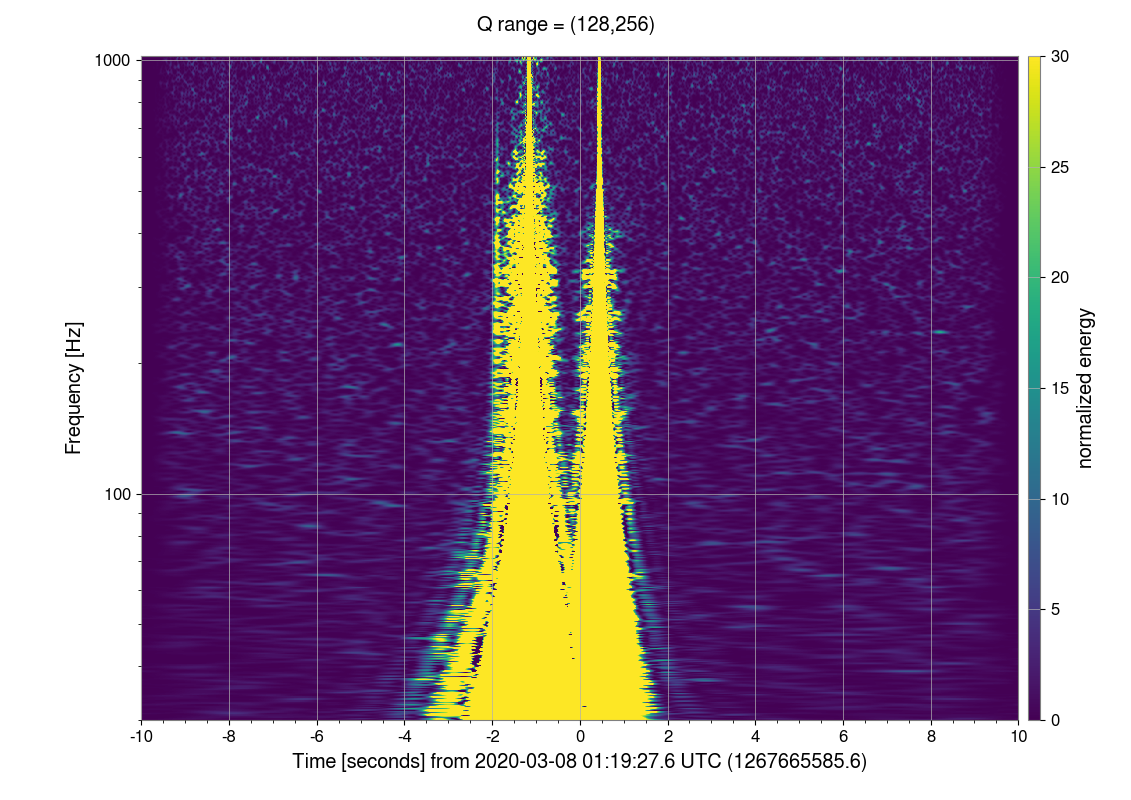
\includegraphics[width=1.2\linewidth]{sectionMBTA/1267665585.60_3.png}
  \end{minipage}
  \hfill
  %
  \begin{minipage}{0.45\linewidth}
    \centering
    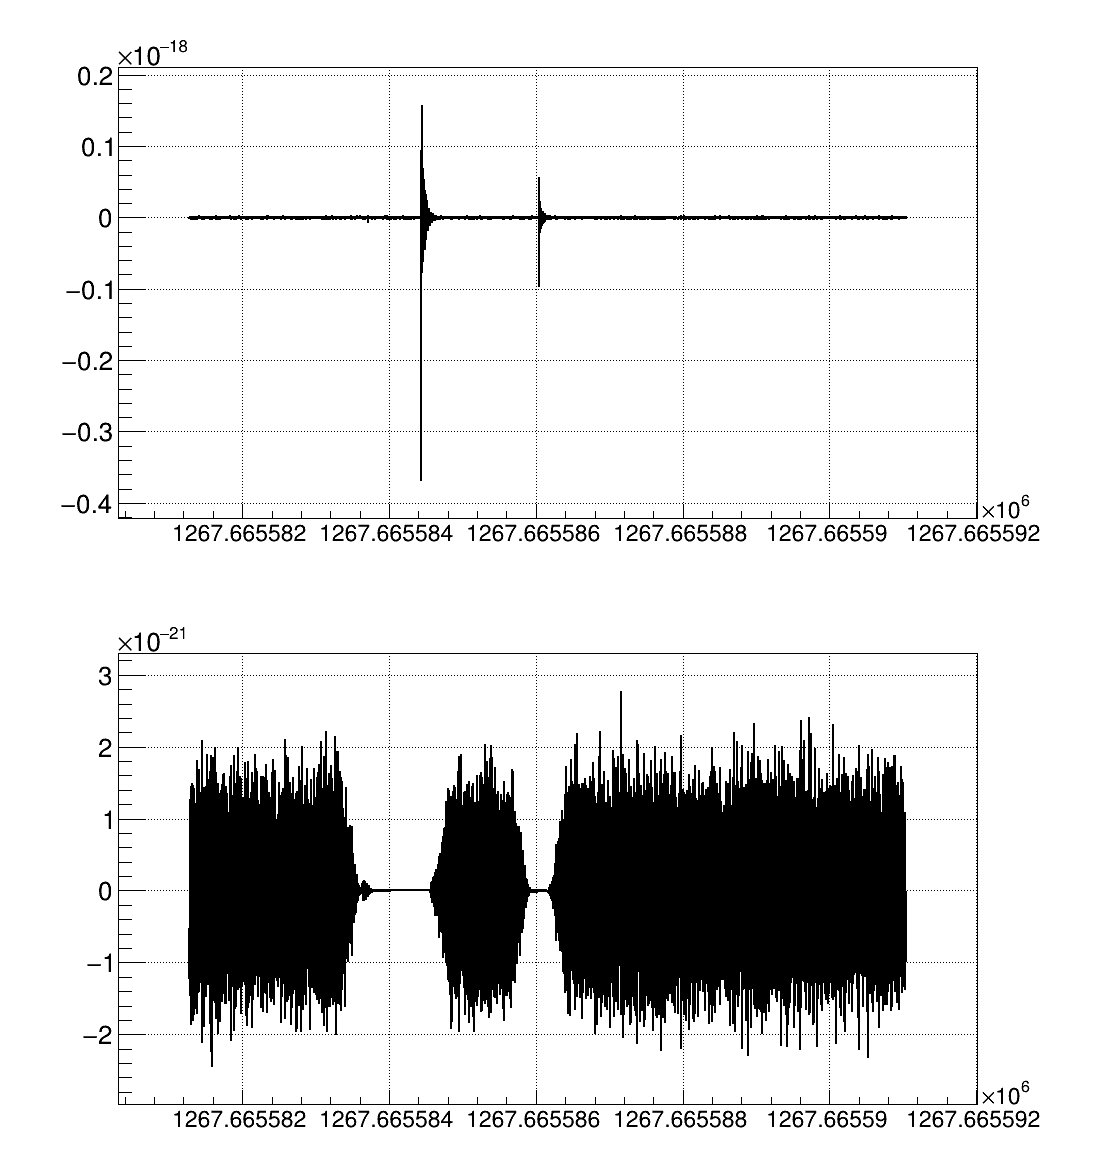
\includegraphics[width=0.9\linewidth]{sectionMBTA/StrainGated.png}
  \end{minipage}
  \caption{Left: Spectrogram around two glitches in L1. Right: strain before (top) and after (bottom) gating around these glitch.}
  \label{fig:strain_gated}
\end{figure}
%
\begin{figure}[ht]
  \centering
  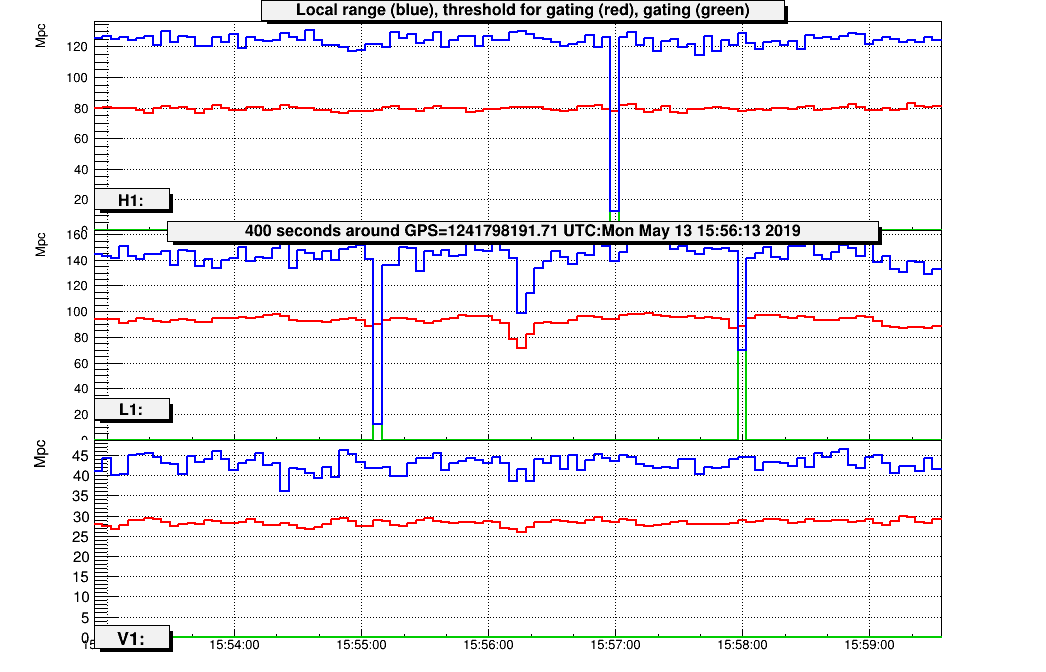
\includegraphics[width=0.65\textwidth]{sectionMBTA/GatingZoom.png}
  \caption{Example of the range (blue) and threshold (red) for gating over time for a segment of O3. The green line indicates gated times.}
  \label{fig:range_glitch}
\end{figure}
%




%%%%%%%%%%
\subsection{Matched Filtering}
\label{sec:matched_filter}
%
% interesting paper: https://arxiv.org/pdf/gr-qc/0509116.pdf
%

The matched filtering technique is the optimal detection strategy in the presence of stationary noise \cite{signal_detection}.
The performance of the filter is caracterized by the signal-to-noise ratio at its output.\\
Let $n(t)$ be the stationary Gaussian noise for a detector.\\
The signal at the output of the detector is 
\begin{equation}
    s(t) = n(t) + h(t)
\end{equation}
where $h(t)$ is the possible astrophysical signal.

The principle of the matched-filtering technique is to compute the correlation of the detector output $s(t)$ with expected GW  waveforms called templates, weighted by the PSD.
If a signal matching the template is mixed with the detector noise, then the correlation will be high.
To increase the chances of detection, many templates are prepared in advance for the filtering in a way that covers a large parameter space.\\
%The matched filtering for gravitational waves analysis is usually done in frequency domain to be computationally effective to easily weight the different frequency contributions to the signal by the noise Power Spectral Density (PSD) of the detector.\\
From \cite{extract_signal}, we can write the filter output for the correlation between $s(t)$ and a template $h_{\textrm{template}}(t)$ in the presence of signal as
%
\begin{align}
  M(t) &=\frac{1}{2\pi} \int_{-\infty}^{+\infty} \tilde{s}(\omega)\tilde{h}_{\textrm{template}}^*(\omega) e^{i\omega t} d\omega\\
  &= \frac{1}{2\pi} \int_{-\infty}^{+\infty} \tilde{n}(\omega)\tilde{h}_{\textrm{template}}^*(\omega) e^{i\omega t} d\omega + \frac{1}{2\pi} \int_{-\infty}^{+\infty} \tilde{h}(\omega)\tilde{h}_{\textrm{template}}^*(\omega) e^{i\omega t} d\omega\\
  &= \nu(t) + \eta(t)\\
\end{align}
%
where $\nu(t)$ is the filter output for the noise and $\eta(t)$ the output for the signal we are looking for.
The noise being a random process it follows from Wiener-Khinchin theorem \cite{extract_signal} that
%
\begin{equation}
  \overline{n^2(t)} = \frac{1}{2\pi} \int_{-\infty}^{+\infty} S_n(\omega) e^{i\omega t}d\omega
\end{equation}
%
where $\overline{n^2}$ is the average noise power and $S_n(f)$ the PSD of the noise.
Therefore the noise power at the output of the filter will be
%
\begin{equation}
  \overline{\nu^2(t)} = \frac{1}{2\pi} \int_{-\infty}^{+\infty} \left| \tilde{h}_{\textrm{template}}^*(\omega) \right|^2 S_n(\omega)e^{i\omega t}d\omega
\end{equation}
%
We define the Signal-to-Noise Ratio (SNR) time series for a signal $s(t) = n(t) + h(t)$ (with $n(t)$ stationnary and Gaussian) and a template $h_{\textrm{template}}(t)$ as
%
\begin{align}
  \rho(t) &= \frac{\eta^2(t)}{\overline{\nu^2}}\\
  & = \frac{1}{2\pi} \frac{ \left| \int_{-\infty}^{+\infty} e^{i\omega t} \tilde h_{\textrm{template}}^*(\omega) \tilde{h}(\omega) d\omega \right|^2 }{ \int_{-\infty}^{+\infty} \left| \tilde{h}_{\textrm{template}}^*(\omega) \right|^2  S_n(\omega) e^{i\omega t} d\omega }
\end{align}
%
Our goal is to have maximal SNR, to this end we search the template which achieves this.
Using Cauchy-Schwartz inequality for square-integrable complex-valued functions, we can write
%
\begin{equation}
  \left| \int_{-\infty}^{+\infty} e^{i\omega t} \tilde h_{\textrm{template}}^*(\omega) \tilde{h}(\omega) d\omega \right|^2 \leq \int_{-\infty}^{+\infty} e^{i\omega t} \left| \tilde h_{\textrm{template}}^*(\omega) \right|^2 d\omega  \int_{-\infty}^{+\infty} e^{i\omega t} \left|\tilde{h}(\omega) \right|^2 d\omega
\end{equation}
%
the maximal SNR value is therefore reached when we attain equality, that is when the template is proportional to the signal: $\tilde h_{\textrm{template}} = \textrm{constant} \times \tilde{h}(\omega)$.
In practice the noise of the detector is neither Gaussian nor stationnary and the template does not reproduce perfectly the signal but we can achieve high precision with fine enough grid of templates (see section \ref{sec:param_space}).

Since the phase of the gravitational wave at merger time $\Phi_0$ is not known we want to maximize the SNR over the phase.
To this end the SNR time series is decomposed into in-phase $h_P$ and in-quadrature $h_Q$ components
%
\begin{equation}
  \rho(t) = \rho_P(t)\cos\Phi_0 + \rho_Q(t)\sin\Phi_0
\end{equation}
%
such that $\rho_P = \rho(\Phi_0=0)$, $\rho_Q = \rho(\Phi_0=\pi/2)$.
This decomposition is related to the polarization of the wave as at merger time $\rho_P$ and $\rho_Q$ are equal to the cross and plus polarizations respectively.
In order to maximize over the phase we have to solve $\rho'(\Phi_{0,best})=0$.
The solution to this equation is
%
\begin{equation}
  \Phi_{0,best} = \tan^{-1} \frac{\rho_Q}{\rho_P} = arg(\rho_P+i\rho_Q)
\end{equation}
%
Putting this back into the expression of $\rho(t)$ yields
%
\begin{equation}
  \rho^2(\Phi_{0,best}) = \rho^2_P + \rho^2_Q
\end{equation}
%
This leads us to define the complex SNR time series
%
\begin{equation}
  Z = \rho_P +i\rho_Q
\end{equation}
%
and the SNR is taken as
%
\begin{equation}
  \text{SNR}^2 = \left| Z \right|^2 = \rho^2_P + \rho^2_Q = \rho^2(\Phi_{0,best})
\end{equation}
%
We call matched-filtering output (MFO) the SNR time series.
In practice we naturally deal with discrete series instead of integrals.
Figure \ref{fig:ex_mfos} shows the matched filtering output for a BNS astrophysical signal.

\begin{figure}[ht]
  \centering
  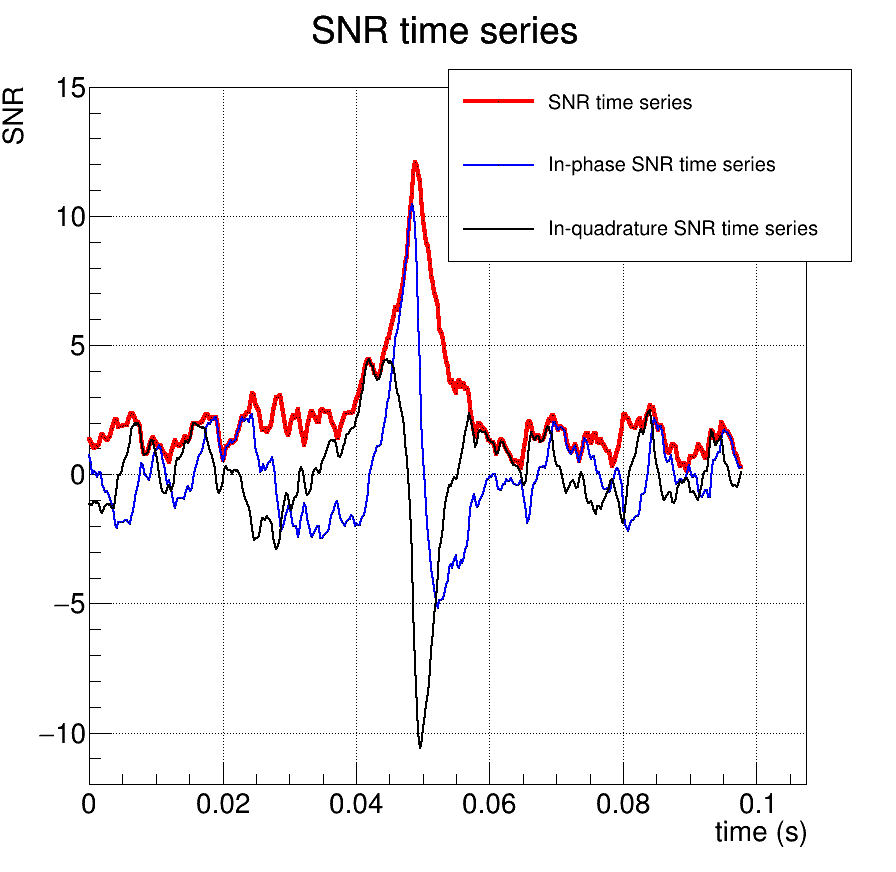
\includegraphics[width=0.5\textwidth]{sectionMBTA/cMfo.png}
  \caption{Matched filtering output for a BNS event (GW190425) with SNR 12.07 in L1}
  \label{fig:ex_mfos}
\end{figure}

%%%%%%%%%%
\subsection{PSD computation}
\label{sec:psd_compute}
The PSD used in the matched filtering should be accurately estimated to have a proper estimation of the background and therefore of the significance of any trigger.
Since high frequency (HF) and low frequency (LF) templates have different duration (the low frequency part of the signal is much longer), the PSD is computed separately for each frequency band.
The computation in MBTA is done using the FFTW3 \cite{FFTW3} implementation of the ``real to half-complex'' FFT.
To limit the bias due to possible noise fluctuations, the PSD used for the matched filtering is the median PSD computed over a user-defined number of FFT.
When running MBTA the PSD is first initialized either by loading the Amplitude Spectral Density (ASD) from a previous MBTA run or by loading a detector strain data file and computing the PSD using this file.
Note that some additional steps can be done when computing the PSD:
\begin{itemize}
\item smoothing of the ASD by averaging some frequency bins together,
\item canceling of some frequency bands if some are known to be noise-polluted: we know for instance that right after the lock of an interferometer, the suspension fibers' transversal mechanical modes of vibration (so-called ``violin modes'') can cause a lot of triggers.
  Canceling the frequency band (like $\SI{512}{Hz} \pm \SI{7.5}{Hz}$ in L1) associated to those modes avoids bad triggers at those times.
\item application of a high-pass shaping filter, a common one being a Butterworth filter of order 4 and cut-off frequency \SI{40}{\hertz} for instance.
  A high-pass filter reduces the signal dynamic and limits numerical issues which would pollute the FFT.
  The filter is applied in time domain to the strain data, the inverse filter is applied in frequency domain.
\end{itemize}
Estimations of the SNR$^2$ sharing between the bands and of the low/high frequency cutoffs to have close to 100\% of the SNR are also done at initialisation of the PSD.

Since the noise in the LIGO and Virgo detectors is not sationnary, the PSD computed at initialization will not properly caracterize the noise at a later time and it should therefore be updated over time, as shown by figure \ref{fig:psd_time}.
As a typical example, during the test performed to prepare the O4 online configuration, FFTs were computed every 4 seconds over \SI{87.5}{s} for the LF band and over \SI{8}{s} for the HF band.
The median PSD was computed over \SI{4000}{s} for the LF band and \SI{1000}{s} for the HF band.
This means roughly over 90 and 250 FFT respectively (acounting for an overlap of 50\% between consecutive FFTs).
The computation of the median PSD can be very time consuming and was therefore updated every 18 (50) FFT for the LF (HF) band.
Meaning that we compute a new median each time 1/5 of the FFTs were updated.
Since the PSD does not fluctuate so fast this choice allows to have a good accuracy in accounting the noise fluctuations while not being too computationally expensive.

\begin{figure}[ht]
  \centering
  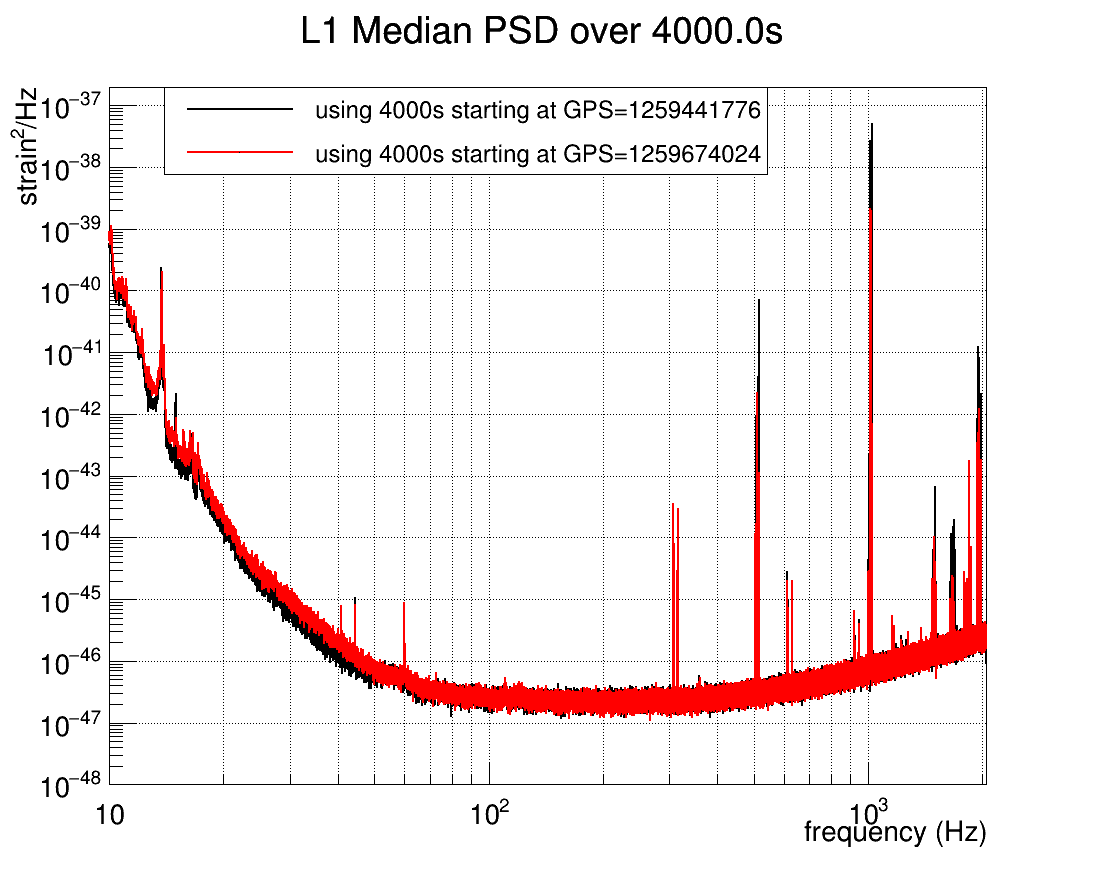
\includegraphics[width=0.6\linewidth]{sectionMBTA/cComparePSD3.png}
  \caption{Difference in the PSD of LIGO Livingston computed over \SI{4000}{s} few days apart.}
  \label{fig:psd_time}
\end{figure}



%%%%%%%%%%
\subsection{Frequency range of the search}
To detect signal in the $h(t)$ data stream we first need to decide the frequency range we want to probe.
The larger the frequency band of the search, the higher the chance to find a signal because the SNR integrated over the band will be higher (for an actual astrophysical event).
But a wider band also requires more computing time.
Furthermore, most of the SNR is collected in a limited frequency band.

To choose the start and end frequency of the search, we compute the SNR loss for several values of them.
The computation depends on the PSD of the detector and the mass of the system considered since the maximum frequency of the signal decreases when the mass of the binary increases.
Figure \ref{fig:start_freq} shows the SNR loss as a function of the starting and end frequency of the search, in H1 and L1, for a \SI{1.4}{\msun}+\SI{1.4}{\msun} BNS system.
Figure \ref{fig:start_freq_mass} shows the same for several masses computed at the same O4 time.
The plots were produced using O3 strain data from GPS = 1268100004 to GPS = 1268100800 (March 13 2020) and O4 strain data from GPS = 1370500020 to GPS = 1370500800 (June 11 2023).

Usually, the starting frequency is chosen at \SI{24}{Hz}.
We see that going below would only allow to recover less than 1\% of the SNR.
It would however result in higher computing cost and is therefore not interesting.
This may change for future runs with the expected detector improvements at low frequency. 

Figure \ref{fig:nuLSO} shows that the frequency at the last stable orbit for low mass systems can go up to a few kilohertz.
Although figure \ref{fig:start_freq} shows that stopping at \SI{1024}{Hz} would allow to recover the quasi-totality of the SNR, the end frequency of the search is typically chosen at \SI{2048}{Hz}.
This an empiric choice motivated by the fact that extending the search to a higher frequency yielded better results in terms of timing resolution.

%
\begin{figure}[hb]
  \centering
  \begin{minipage}{0.95\linewidth}
    \centering
    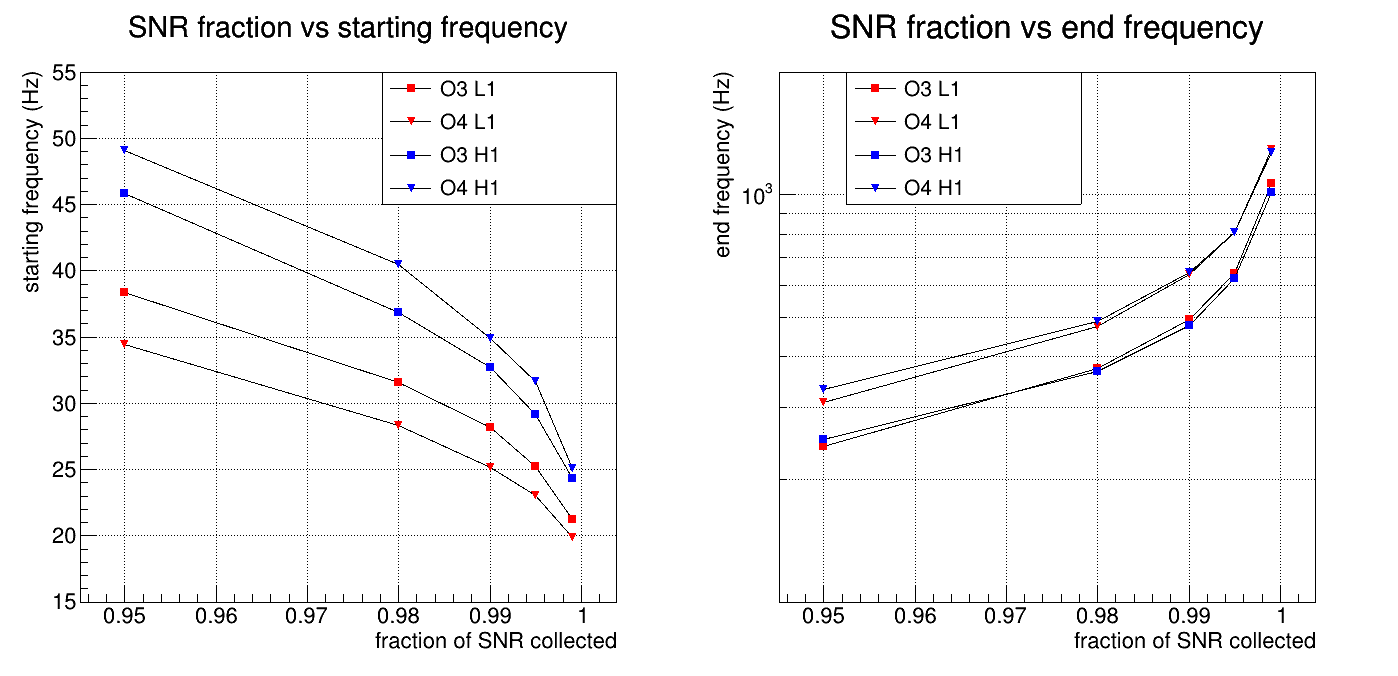
\includegraphics[width=\linewidth]{sectionMBTA/cSnrFreqO3O4.png}
    \captionof{figure}{Fraction of SNR collected as a function of the starting frequency (left) and end frequency (right) of the search, respectively assuming an end frequency of \SI{2048}{Hz} and start frequency of \SI{10}{Hz}.}
    \label{fig:start_freq}
  \end{minipage}

  \begin{minipage}{0.95\linewidth}
    \centering
    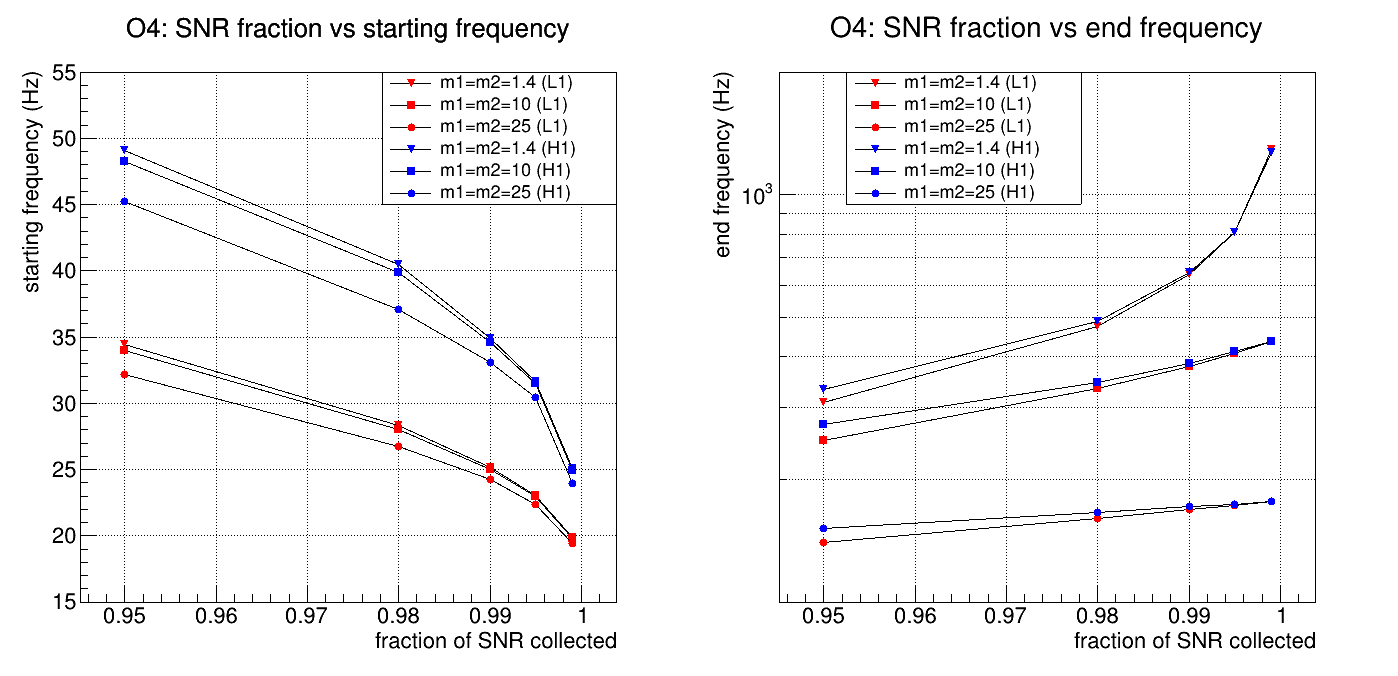
\includegraphics[width=\linewidth]{sectionMBTA/cSnrFreqMassO4.png}
    \captionof{figure}{Fraction of SNR collected using an O4 PSD for several masses as a function of the starting frequency (left) and end frequency (right) of the search, respectively assuming an end frequency of \SI{2048}{Hz} and start frequency of \SI{10}{Hz}.}
    \label{fig:start_freq_mass}
  \end{minipage}
\end{figure}


% \begin{figure}[hb]
%   \centering
%   \begin{minipage}{0.95\linewidth}
%     \centering
%     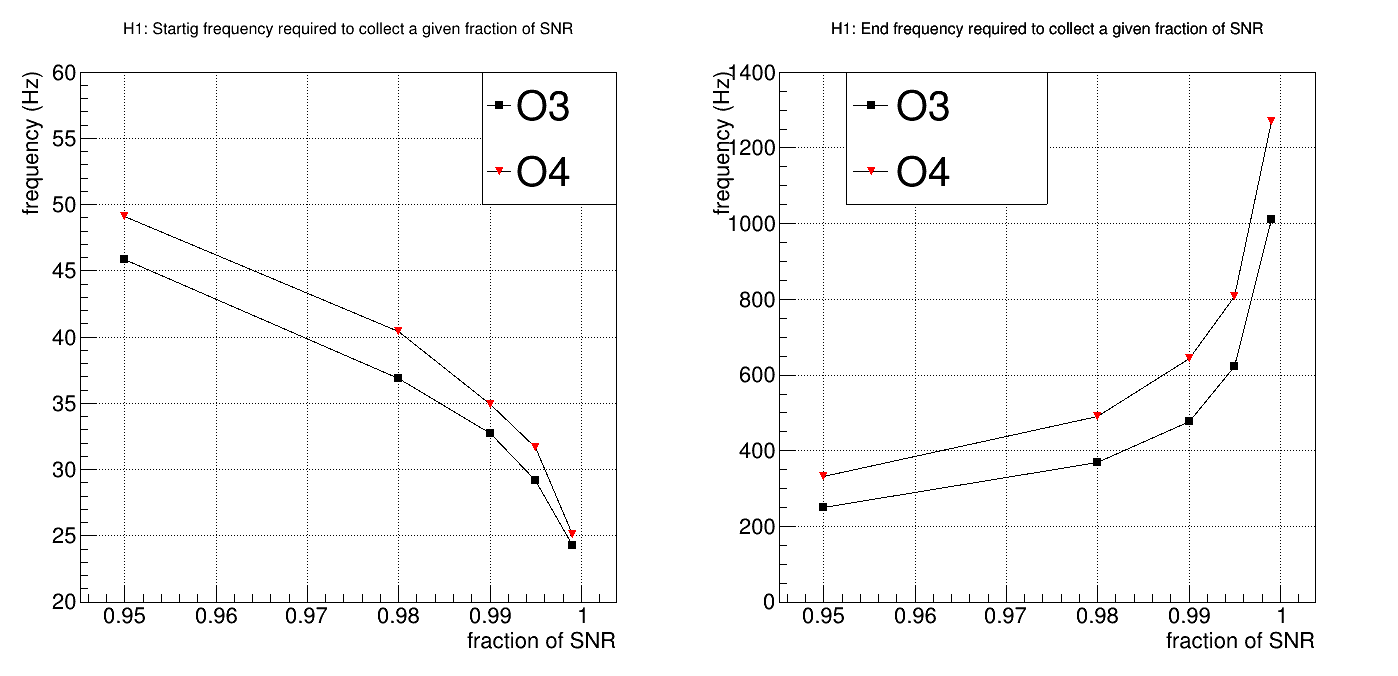
\includegraphics[width=\linewidth]{sectionMBTA/cSnrFreqO3O4_H.png}
%     \captionof{figure}{Fraction of SNR collected as a function of the starting frequency (left) and end frequency (right) of the search, respectively assuming an end frequency of \SI{2048}{Hz} and start frequency of \SI{10}{Hz} in H1.}
%     \label{fig:start_freq_H1}
%   \end{minipage}

%   \begin{minipage}{0.95\linewidth}
%     \centering
%     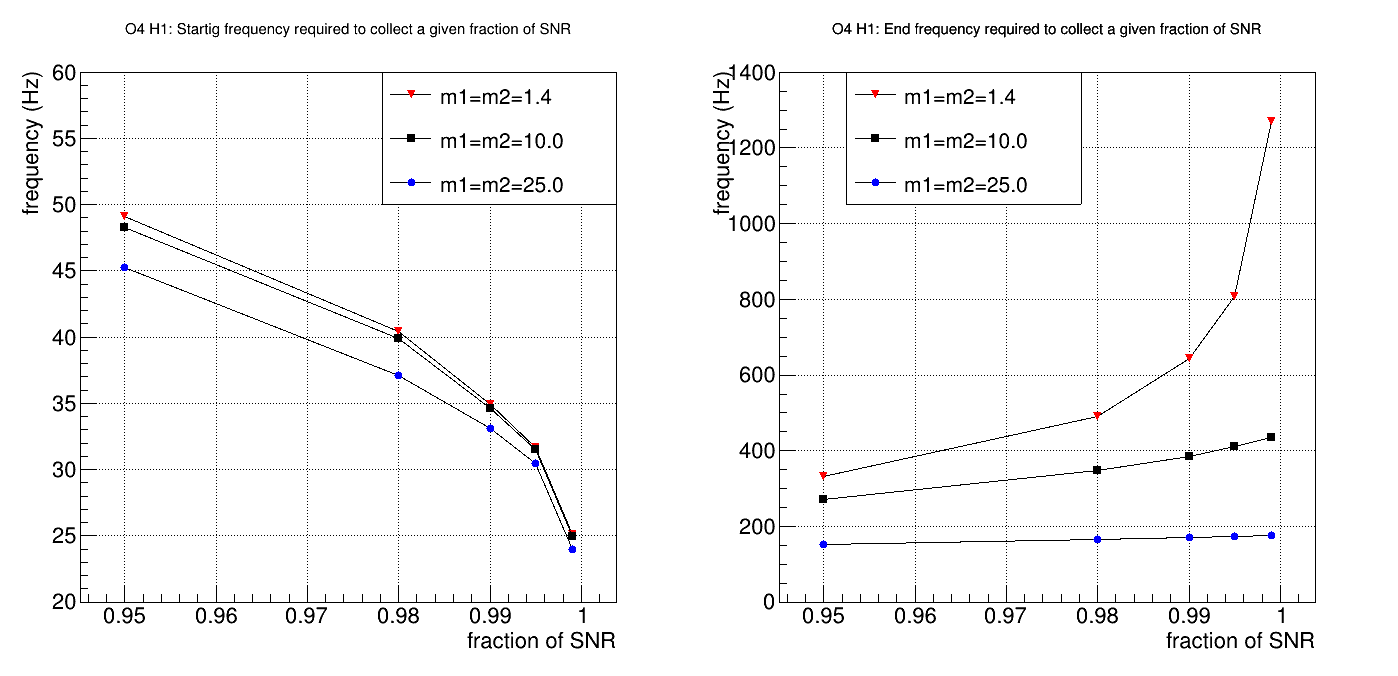
\includegraphics[width=\linewidth]{sectionMBTA/cSnrFreqMassO4_H.png}
%     \captionof{figure}{Fraction of SNR collected for several masses as a function of the starting frequency (left) and end frequency (right) of the search, respectively assuming an end frequency of \SI{2048}{Hz} and start frequency of \SI{10}{Hz} in H1.}
%     \label{fig:start_freq_mass_H1}
%   \end{minipage}
% \end{figure}

\begin{figure}
  \centering
  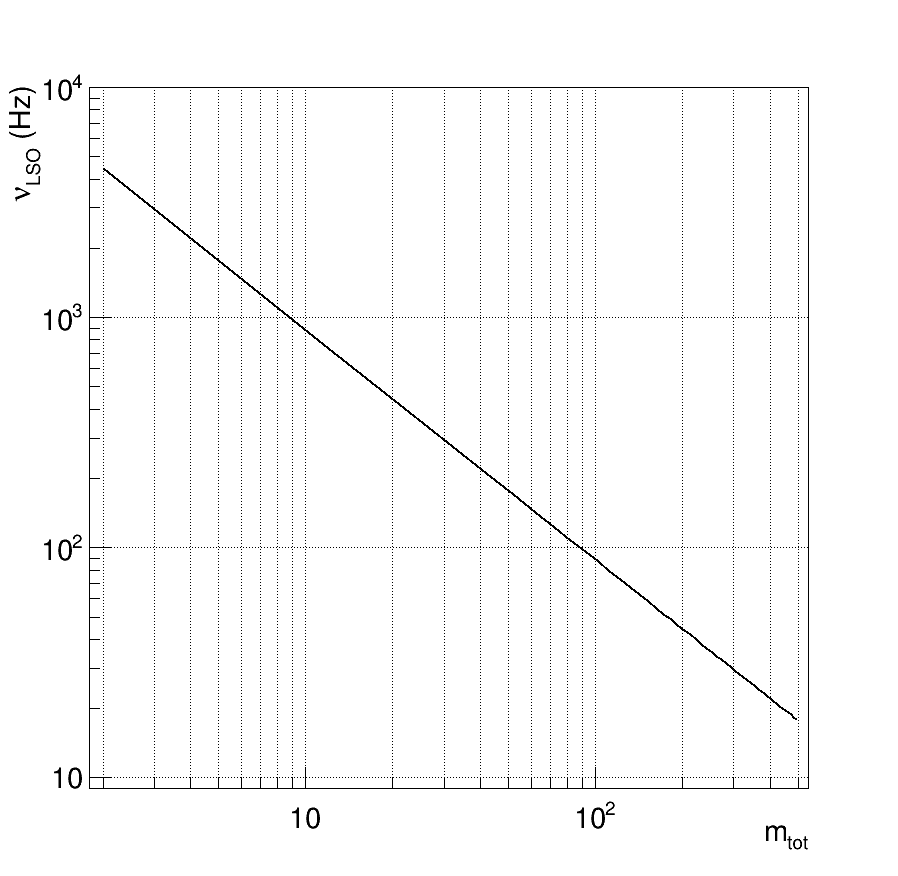
\includegraphics[width=0.5\linewidth]{sectionMBTA/cNuLSO.png}
  \caption{Signal frequency at the last stable orbit as a function of the total mass (see eq. \ref{eq:f_isco}).}
  \label{fig:nuLSO}
\end{figure}


%%%%%%%%%%
\clearpage \newpage
\subsection{Multi-band analysis}
\label{sec:2bands}

As mentionned previously, the filtering is done in two separate frequency bands.
The splitting frequency can be chosen such that the SNR squared is roughly equally shared between the two bands.
This is typically achieved by splitting frequencies around \SI{100}{\hertz} for a BNS system.
In practice, an empiric choice is to generally have slightly more SNR in the high frequency band with a splitting frequency at \SI{80}{Hz}.
This is because the search is run with the same splitting frequency for a large part of the parameter space.
Having a bit more SNR in the HF band when computed for BNS, provides more high mass templates with appropriate signal in the HF band.
Another consideration is the impact of the  different shape of the detector sensitivity, which means different SNR per frequency band.
Since the spliting frequency must be the same for all detectors in the current MBTA implementation, this splitting is done on the most sensitive detector, L1 for O3 and O4.
For instance during the first weeks of O4 the expected SNR$^2$ sharing was 46\% for the HF band and 54\% for the LF band in L1, and 30\% for the HF band and 70\% for the LF band in H1.
Figures \ref{fig:O3_snr_sharing_inj} to \ref{fig:O3_snr_sharing_Gaus} show the SNR sharing for singles detector triggers obtained during an analysis of data with injected simulated signals (see section \ref{sec:inj}), for O3 single detector triggers respectively and for triggers obtained on Gaussian noise.
For O3 single detector triggers, the SNR seems larger in the low frequency band.

\begin{figure}[ht]
  \centering
  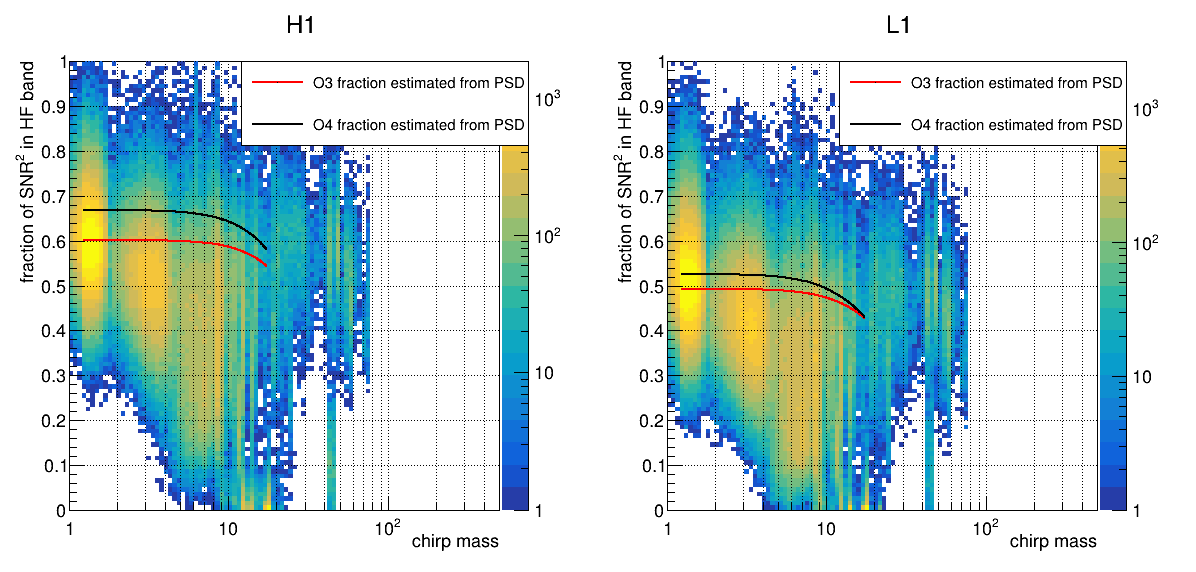
\includegraphics[width=\textwidth]{sectionMBTA/cSnrFracMchirpInj.png}
  \caption{Fraction of SNR$^2$ in the HF band as a function of the chirp mass for O3 common injections on top of O3 data (section \ref{sec:inj}) analyzed with the pipeline O3 configuration. The expected fraction is also plotted for O3 and O4.}
  \label{fig:O3_snr_sharing_inj}
\end{figure}

\begin{figure}[ht]
  \centering
  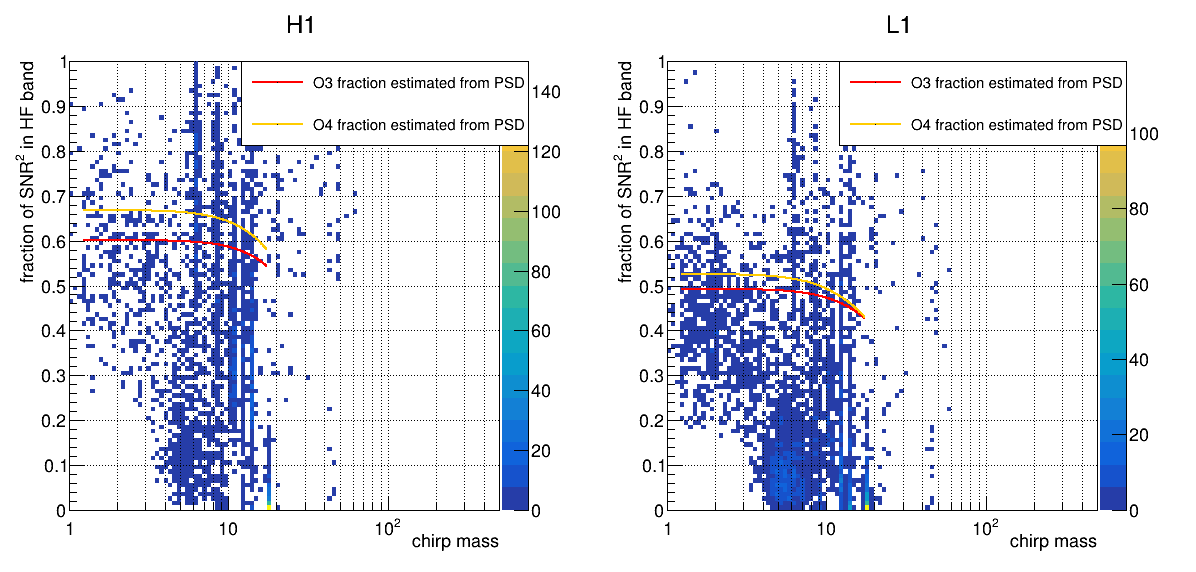
\includegraphics[width=\textwidth]{sectionMBTA/cSnrFracMchirp.png}
  \caption{Fraction of SNR$^2$ in the HF band as a function of the chirp mass for O3 single detector triggers analyzed with the pipeline O3 configuration having a rwSNR larger than 8. The expected fraction is also plotted for O3 and O4.}
  \label{fig:O3_snr_sharing}
\end{figure}

\begin{figure}[ht]
  \centering
  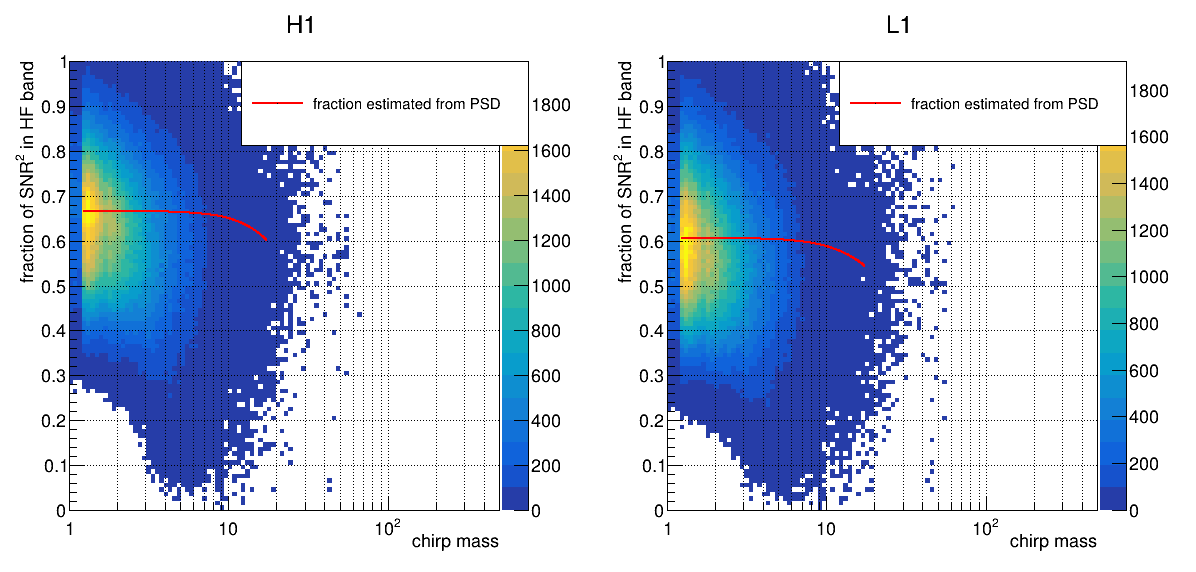
\includegraphics[width=\textwidth]{sectionMBTA/cSnrFracMchirpGaus.png}
  \caption{Fraction of SNR$^2$ in the HF band as a function of the chirp mass for single detector triggers obtained on simulated Gaussian strain (see section \ref{sec:gaussian_noise}) analyzed with the pipeline O3 configuration. The expected fraction is also plotted for the PSD used to generate the strain.}
  \label{fig:O3_snr_sharing_Gaus}
\end{figure}

Summarizing the discussion on the starting, end and split frequencies, the bands are chosen as:
%
\begin{itemize}
\item a low frequency band ranging from \SI{24}{\hertz} to \SI{80}{\hertz},
\item a high frequency band ranging from \SI{80}{\hertz} to \SI{2048}{\hertz}.
\end{itemize}

\subsubsection{Combining bands}

The result of the matched filtering in the two frequency bands is coherently summed following
%
\begin{align}
  \textrm{SNR}(t,\textrm{template}) =& \int_{\omega_{min}}^{\omega_{max}} \tilde{s}(\omega)\tilde{h}_{\textrm{template}}^*(\omega) e^{i\omega t} d\omega\\
  =& \int_{\omega_{min}}^{\omega_{split}} \tilde{s}(\omega)\tilde{h}_{\textrm{template}}^*(\omega) e^{i\omega t} d\omega + \int_{\omega_{split}}^{\omega_{max}} \tilde{s}(\omega)\tilde{h}_{\textrm{template}}^*(\omega) e^{i\omega t} d\omega
\end{align}
%
to get the SNR time series.

An interpolation of the low-frequency band MFO is needed before combining with the high-frequency band MFO due to the difference in sampling rate between the two bands.
Accounting for the time and phase shift the individual bands MFOs are recombined following
%
\begin{align}
  &\rho_P(t) = \rho_{LF,P}(t) + \cos(\Delta\phi)\rho_{HF,P}(t+\Delta t) - \sin(\Delta\phi)\rho_{HF,Q}(t+\Delta t)\\
  &\rho_Q(t) = \rho_{LF,Q}(t) + \sin(\Delta\phi)\rho_{HF,P}(t+\Delta t) + \cos(\Delta\phi)\rho_{HF,Q}(t+\Delta t)
    \label{eq:mfo_combi}
\end{align}
%
$\Delta t$ is the time it takes for the signal to go from the low-frequency band to the high-frequency band (i.e. the time ``spent'' in the low-frequency band), $\Delta\phi$ is the phase offset of the signal between the two bands.
Both typically depend on the templates for each band, as well as the full band template we want to emulate and are computed at the initialization of the pipeline.
Figure \ref{fig:mfo_combi} shows the low frequency, high frequency and combined MFOs for an astrophysical event.\\

\begin{figure}
  \centering
  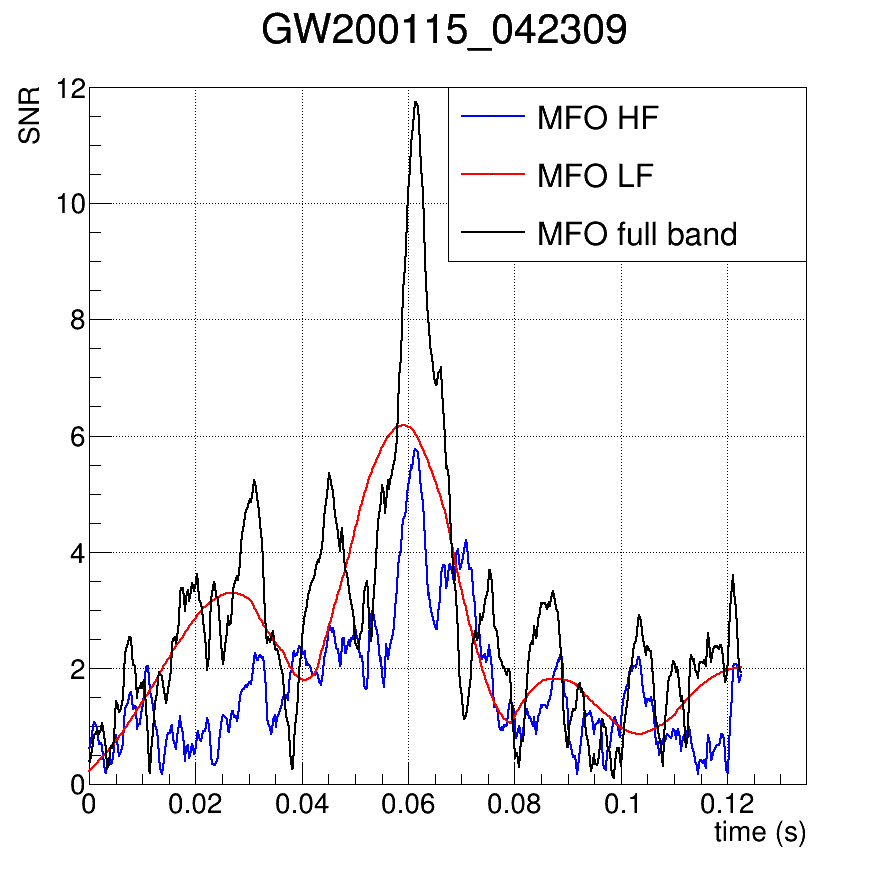
\includegraphics[width=0.6\linewidth]{sectionMBTA/cMFOcombi.png}
  \caption{Matched Filtering Outputs (MFOs) for the LF, HF and full frequency band for astrophysical event GW200115\_042309 detected on O3-replay data using MBTA O4 configuration.}
  \label{fig:mfo_combi}
\end{figure}

Analyzing the detector strain in two frequency bands implies that we have templates for each frequency band.
The templates used for the filtering are called real templates (RT).
MBTA has therefore two RT banks, one for each band.
To describe the full waveform after combination of the band MBTA uses an additional bank of virtual templates (VT).
When claiming a detection, the parameters announced for the source are those of the VT with the best match.

We do not have the same number of templates for each frequency bands, meaning that the templates do not share exactly the same parameters either.
To properly combine the result of the matched filtering of each bands, we need to be able to tell which templates of the LF bands are compatible with which templates of the HF band to form a VT.
This is done using a modified version of the PyCBC ``banksim'' algorithm \cite{banksim} by injecting each template of the VT bank as a signal in the data and finding the RT which best match each VT.
This allows us to have for each VT the combination of RTs that match it best.
A same RT can be combined to form several VTs, leading to a reduction of usually more than an order of magnitude in the number of RT compared to the numbers of VT.




%%%%%%%%%%
\subsection{MBTA parameter space and template bank generation}
\label{sec:param_space}

We need to build templates to filter the $h(t)$ data.
%In the case of CBC searches the parameter which is best recovered is the chirp mass (eq. \ref{eq:mchirp}).
%It largely dictates the amplitude and duration of the waveform.
%Similarly the effective spin (eq. \ref{eq:spin_eff}) influences the duration of the waveform.\textcolor{red}{Je ne comprend pas le besoin de passer par la chirp mass.
%Il faudrait expliquer pourquoi on prend ces limites}
%These two quantities are computed from the masses and spins of the two objects of the binary.
%Their values are degenerate, thus building a bank using only these two parameters would not allow to measure precisely the individual masses and spins.
For CBC searches parameter space, we consider the masses and spins of the objects of the binary.
The parameters are the observed ones and therefore in the detector frame (i.e. redshifted masses).
Only the cases of either aligned or anti-aligned spins are considered in all searches.
It was shown that considering misaligned spins does not improve significantly the detection rate \cite{gw150914,bank_spin}.

%During O3, MBTA's parameter space covered the range $\left[1\msun, 195\msun \right]$ for the masses, with $m_1 + m_2 \leq 200\msun$.
%The spins were limited to $\left[-0.05,0.05\right]$ below $2\msun$ and $\left[-0.997,0.997\right]$ otherwise.
%For O4 the mass range was extended from $195\msun$ to $500\msun$ with $m_1/m_2 \leq3$.
%Spins considerations are the same.
During O3, MBTA's parameter space covered masses up to \SI{195}{\msun}.
In preparation for O4, the mass range of the parameter space was extended up to \SI{500}{\msun}.
The spins consideration were kept the same.
A new algorithm was used by the Urbino group to generate the template bank. 

A template bank for a sub-solar mass (SSM) search was also created for the O3 offline analysis and adjusted for the O4 online analysis.
The SSM search, lead by the IP2I in Lyon, considers CBC signals with at least one component of the binary lighter than 1 \msun.
Considered masses are $m_1 \in \left[ 0.2, 10 \right]$\msun, $m_2 \in \left[ 0.2, 1 \right]$\msun with $m_1/m_2 \in \left[ 1,10 \right]$\msun.
Spins are limited to $\left[ -0.1,0.1 \right]$ for masses below $0.5\msun$ and $\left[ -0.9,0.9 \right]$ otherwise.

%Waveforms are generated using accurate models which rely on several physical theories and techniques (effective-one-body theory \cite{EOB}, numerical relativity \cite{NR}, black-hole pertubation theory \cite{BH_perturbation}...) \textcolor{red}{Pas sûr qu'il faille en parler ici puisque plus loin tu donnes l'info détaillés}.


\subsubsection{MBTA's O3 main template bank}
\label{sec:bankO3}

During O3, MBTA ran the main search in parallel on three independent parts of the parameter space.
They were named region 1, 2 and 3 and corresponded to what we can expect roughly in terms of parameters for BNS, NSBH and BBH respectively.
This includes region between 2 and 5 \msun where the separation between NS and BH is unclear.
The bank of template for region 1 had low masses and small spins: $$1 \msun \leq m_{1,2} \leq 2 \msun$$  $$|s_{1,2}|<0.05$$
For region 2 the parameter space was defined as $$1 \msun \leq m_{1} \leq 2 \msun, |s_{1}|<0.05 \textrm{ for what could be a neutron star,}$$  $$2 \msun \leq m_{2} \leq 99 \msun, |s_{2}|<0.997 \textrm{ for what could be a black hole.}$$
Region 3 included templates with $$2 \msun \leq m_{1,2} \leq 195 \msun,$$ $$m_1+m_2 \leq 200 \msun,$$ $$|s_{1,2}|<0.997\text{ .}$$

The limit of \SI{2}{\msun} is fairly small for expected BNS, but it allows for objects with high spin as light as \SI{2}{\msun}.
Region 1 was generated using the TaylorF2 approximant \cite{taylorf2} for the bank generation and SpinTaylorT4 \cite{spintaylort4}  for the analysis.
Region 2 and 3 were both generated using SEOBNRv4\_ROM and SEOBNRv4 \cite{seobnrv4_rom} for the bank generation and analysis respectively.

The templates of the O3 bank were computed starting at a frequency of \SI{25}{Hz}, \SI{23}{Hz} and \SI{21}{Hz} for regions 1, 2 and 3 respectively.

The distribution of the templates in the parameter space depends on the generation algorithm and the parameters used.
One of the most important parameters is the minimal match.
The minimal match is the lowest value allowed for the match between any given waveform and the template that matches the best \cite{Babak_2006}.
In other words, if we construct a bank with a minimal match of 0.97, as for the O3 template bank, for any astrophysical signal with parameters inside our parameter space reaches the detector, the match is expected to be larger than 0.97.
But there could be few cases with slighty smaller match.

The two main types of algorithms for template bank generation are the following:
\begin{itemize}
\item Geometric algorithms which map the parameter space with lattices and place templates from neighbour to neighbour such that neighboring templates have a match close to the minimal match \cite{geometric_bank}.
\item Stochastic algorithms place templates at random within the parameter space and then removes the one that are not necessary, i.e. those that can be removed without dropping the minimal below the requested value \cite{stochastic_bank}.
\end{itemize}
The template bank used by MBTA during O3 was a geometric template bank.
Figure \ref{fig:bankO3} shows the distribution of templates in the 3 regions.
%
\begin{figure}
  \centering
  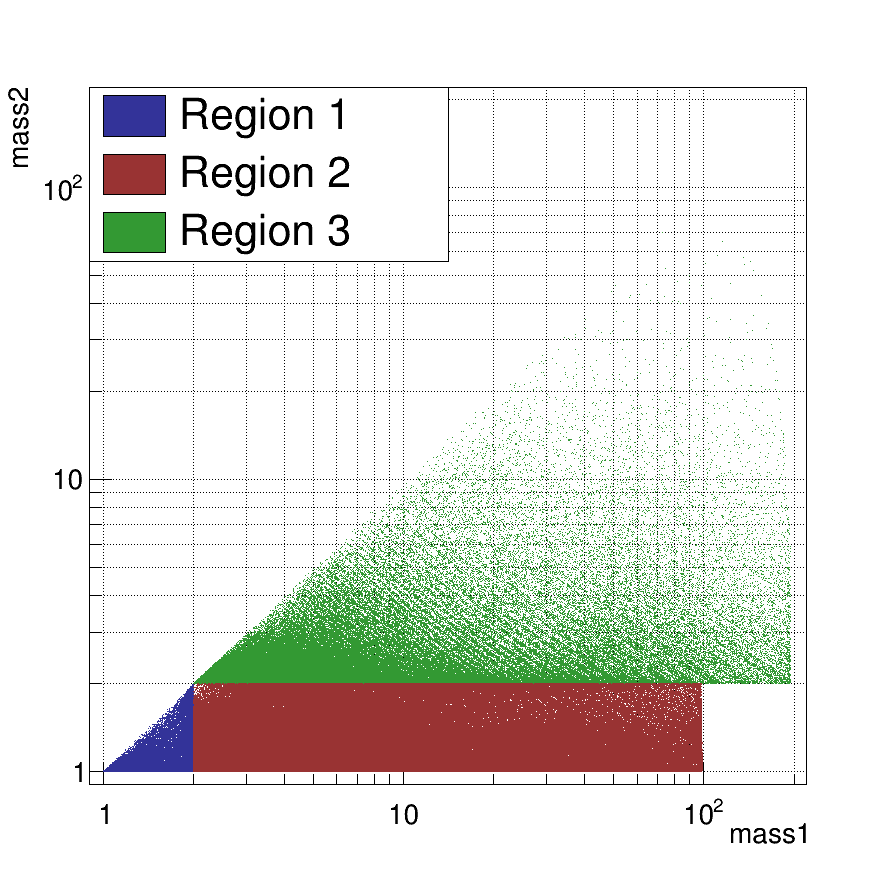
\includegraphics[width=0.5\textwidth]{cBank.png}
  \caption{Template distribution of the template bank used by MBTA during O3}
  \label{fig:bankO3}
\end{figure}
%


\subsubsection{MBTA's O4 template bank}
\label{sec:bankO4}

For O4 MBTA changed completely its template bank.
The parameter space was extended and made of a single region.
Furthermore, a novel template placement algorithm was used.
This algorithm is called hybrid, it is a mix of geometric and stochastic placement.
It starts by initializing a set of randomly placed templates that will act as seeds, one of them is taken to be the starting point for the building of the bank.
From this chosen point templates are placed following a geometric procedure.
Some of them that are ``far-away'' from the seed will then be considered as seed one after the other to repeat the procedure until no new seed can be found.
The procedure is explained in more details in \cite{hybrid1,hybrid2}.

MBTA's O4 bank is created in several steps:
\begin{itemize}
\item First a BNS seed template bank is generated with a geometric placement algorithm and a minimal match of 0.98 .
This BNS seed contains templates with $1 \msun \leq m_{1,2} \leq 3 \msun$ and $|s_{1,2}|\leq 0.05$ for masses below $2 \msun$, $|s_{1,2}| \leq 0.997$ for others.
\item Then a BBH seed is created using the hybrid algorithm, with a minimal match of 0.98, $5 \msun \leq m_{1,2} \leq 500 \msun$, a mass ratio limit $m_1/m_2 \leq 3$ and $|s_{1,2}| \leq 0.997$.
\item The two seeds are eventually used to run the hybrid algorithm and complete the bank with a minimal match of 0.965 .
  The final bank has parameters $m_{1,2} \in [1,500]\msun$, $m_{\text{tot}} \in [1,500]\msun$, $q \in [1,50]$.
  Spin are limited to 0.05 in magnitude for masses below 2\msun, 0.997 otherwise.
\end{itemize}
The minimal match is thus higher in the most interesting regions with the largest source populations.
Figure \ref{fig:bankO4} shows the repartition of the templates in the mass1-mass2 plane and m$_{\text{chirp}}$-$\chi_{\text{eff}}$ planes.

Templates of the BBH seed and full bank with duration larger than \SI{200}{ms} are discarded.
Among the templates generated for the full bank we consider a sub-category: those that have a merging frequency lower than the frequency band separation frequency.
Since in this case the quasi-totality of the signal is in the low frequency band, there is a high chance that the LF RT associated to the VT will likely be combined with a random HF RT.
Any VT with peak frequency smaller than the separation frequency or associated to a LF RT with peak frequency lower than the separation frequency, or to a HF RT with duration below \SI{20}{ms} are therefore run only on one frequency band.
These templates are filtered by the so-called ``job 90''.

The waveform approximant used for the BNS seed are TaylorF2 \cite{taylorf2}  for the bank generation and SpinTaylorT4 \cite{spintaylort4}  for the analysis.
The BBH seed and full bank are both generated using SEOBNRv4\_ROM SEOBNRv4\_opt \cite{seobnrv4_rom} for the bank and analysis respectively.

The templates of the O4 bank are generated starting at a frequency of \SI{25}{Hz} for the BNS seed and \SI{18}{Hz} for the BBH seed and the full bank.

The real template banks are generated in the same way as the VT full bank, with the same parameters but no requirement on the template duration.
RTs are generated for a separation frequency of the bands at \SI{80}{\hertz}.


% \begin{figure}
%   \centering
%   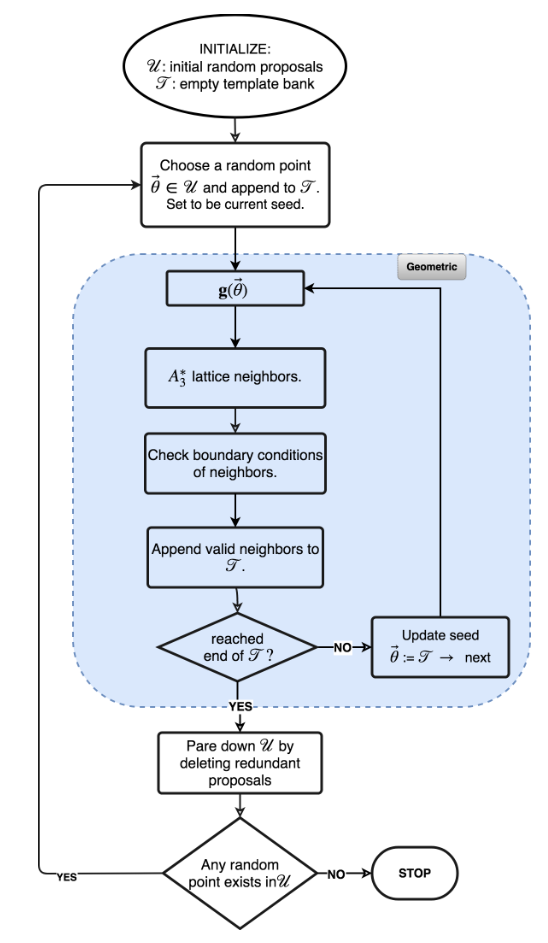
\includegraphics[width=0.4\linewidth]{hybrid_flowchart.png}
%   \caption{Flowchart of the hybrid template bank algorithm taken from \cite{hybrid2}
%   \textcolor{red}{Pas sur que ce soit une figure utile dans cette thèse. Il vaut mieux mettre des figure sur les distribution de template, voir leur durée.}}
%   \label{fig:hybrid}
% \end{figure}


\begin{figure}[ht]
  \centering
  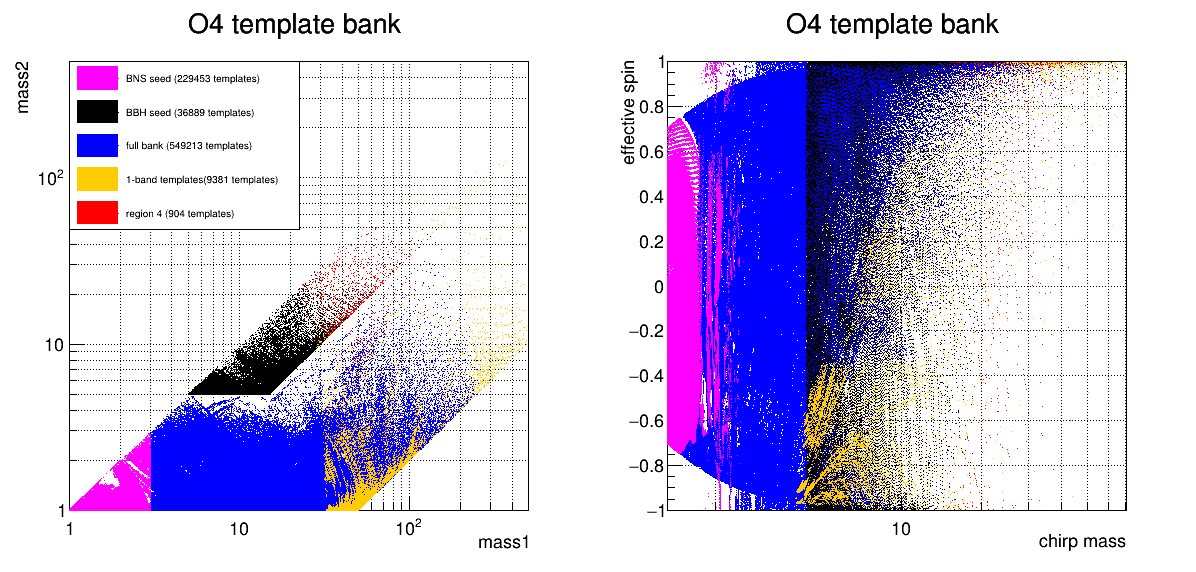
\includegraphics[width=\textwidth]{cBankO4.png}
  \caption{MBTA O4 template bank. Left: mass1 vs mass2. Right: chirp mass vs effective spin.}
  \label{fig:bankO4}
\end{figure}




\subsection{Single detector triggers search}
\label{sec:single_search}
The search for astrophysical signals starts with independent searches in each of the interferometer of the network.
As mentioned previously the matched-filetring of each interferometer data is carried out in two frequency bands.

The matched-filtering being done in the two frequency bands, triggers may arise (when the maximum of the SNR time series goes above a given threshold)  in one or the other.
In this case the combination process (eq. \ref{eq:mfo_combi}) is done using the RTs of the other frequency band for every VT that is associated to the RT of the trigger within a certain time window.
This window is centered on the time of the trigger and its duration depends on the width of the maximum SNR peak of the MFO.
The duration of the window can't exceed \SI{25}{ms}.
If the combined SNR is in turn above a specified threshold we have a \textbf{single detector trigger}.
The two real templates are then recombined on a longer time window to enable parameter consistency tests.

Some triggers produced by noise can sometimes have quite large values of SNR.
In order to identify and reject them some tools were developped.
We present here three of them.

\subsubsection{Signal consistency test: $\chi^2$}
\label{sec:chi2}
Gravitational waves signals have a very specific power distribution in the time-frequency domain.
The role of the $\chi^2$ test presented in this section is to check that the distribution of the signal as a function of the frequency is consistent with what is expected for a GW signal.
The $\chi^2$ was mostly used during O2.
It is a poor version of the \achi (see next section) by which it was surclassed during O3.

A cut on this $\chi^2$ quantity is still applied to triggers during MBTA analysis.
The principle of the $\chi^2$ is to compare the difference in measured SNR  vs theoretical SNR, in-phase and in-quadrature, in each frequency band:
%
\begin{dmath}
  \label{eq:chi2}
  \chi^2 =  \sum_{i=0}^{N_{\textrm{band}}} \left[  \left( \textrm{SNR}_{\textrm{P,meas,}i} - \textrm{SNR}_{\textrm{P,th,}i} \times \alpha_{i} \times \cos\left(\Delta\Phi_{i-1,i} \right)^2 \right)\\
    % 
    + \left( \textrm{SNR}_{\textrm{Q,meas,}i} - \textrm{SNR}_{\textrm{Q,th,}i} \times \alpha_{i} \times \cos\left(\Delta\Phi_{i-1,i} \right)^2 \right) \right]
\end{dmath}
% 
where $\textrm{SNR}_{\textrm{P/Q, meas/th, }i}$ is the measured (meas) or theoretical (th) in-phase (P) or in-quadrature (Q) SNR for each frequency band, $\alpha_{i}$ is the fraction of the SNR in band $i$ and $\Delta\Phi_{i-1,i}$ the phase difference between the frequency bands (0 for $i=0$).
The expected value for the ideal case of an astrophysical signal without noise is, by construction, $\chi^2=0$ as the measured and theoretical SNR would be equal.
In practice a trigger is rejected if its $\chi^2$ is larger than a threshold defined as
%
\begin{equation}
  \chi^2_{cut} = A(2 + B \times \textrm{SNR}^2);
  \label{eq:chi2cut}
\end{equation}
%
with $A = 3$ and $B = 0.025$.

This signal consistency test is not used anymore for O4. 

\subsubsection{\achi and rwSNR}
\label{sec:achi2}

Similarly to the way $\chi^2$ checks for consistent repartition of the SNR in frequency, we can test the consistency of the time evolution of the SNR around its maximum value.
This is done thanks to a quantity call \achi.

The \achi quantifies the mismatch between the measured matched-filtering output (MFO = SNR time series) and the theoretical MFO that is expected from the autocorrelation of the template.
It is computed following:
%%
\begin{equation}
  \label{eq:achi2th}
  \achi = \frac{1}{2\Delta t} \int_{t_0-\Delta t/2}^{t_0+\Delta t/2}\left|\left| \begin{pmatrix} \rho_P \\ \rho_Q \end{pmatrix}
      - \rho_{max} \begin{pmatrix} \cos\Delta\Phi & -\sin\Delta\Phi \\ \sin\Delta\Phi & \cos\Delta\Phi \end{pmatrix} \begin{pmatrix} \rho_{P,th} \\ \rho_{Q,th} \end{pmatrix} \right| \right|
\end{equation}
%%
where $\rho$ is the SNR time series, $\rho_{th}$ is the theoretical SNR time series, $t_0$ the time of the maximum of the SNR time series $\rho_{max}$ (SNR of the event), $\Delta\Phi$ the phase difference between measured and expected SNR time series and $\Delta t$ a time interval centered on $t_0$.

In practice however we deal with discrete series and MFOs, the \achi is then computed on $400$ points following:
%%
\begin{equation}
\label{eq:achi2}
    \achi = \frac{1}{2\textrm{N}} \sum_{i=0}^{\textrm{N-1}} \left[  \left( \textrm{MFO}_{P,meas}[i] - \textrm{Rot}_{P,exp}[i] \right)^2 + \left( \textrm{MFO}_{Q,meas}[i] - \textrm{Rot}_{Q,exp}[i] \right)^2 \right]
\end{equation}
%%
where
\begin{align}
  \textrm{Rot}_{P,exp}[i] &= \cos\Delta\Phi \times \textrm{MFO}_{P,exp}[i] - \sin\Delta\Phi \times \textrm{MFO}_{Q,exp}[i]\\
  \textrm{Rot}_{Q,exp}[i] &= \sin\Delta\Phi \times \textrm{MFO}_{P,exp}[i] + \cos\Delta\Phi \times \textrm{MFO}_{Q,exp}[i]
\end{align}
%%

The \achi is then used to reweight the SNR.
The reweighted SNR (rwSNR) was introduced as a mean to downgrade the significance of triggers that were not consistent with the templated they were matched with.
It is a powerful tool to discriminate background from astrophysical candidates.
The reweighting of the SNR is then done following
%
\begin{equation}
\label{eq:rwsnr}
    \textrm{rwSNR} = \begin{cases}
    \snr, & \textrm{if \achi} \leq 1.\\
    \snr \times \left( \frac{ \textrm{A}+\left[\achi\right]^\alpha }{A+1} \right)^{-\frac{1}{\beta}}, & \text{otherwise}.
  \end{cases}
\end{equation}
%
for O3 the parameters took the values A=10, $\alpha$=5 and $\beta$=8.
Figure \ref{fig:mfo_achi2} shows the measured and expected MFOs for an astrophysical event and a loud noise trigger with the associated \achi values and rwSNR.

%
\begin{figure}[ht]
  \centering
  \begin{minipage}{0.45\linewidth}
    \centering
    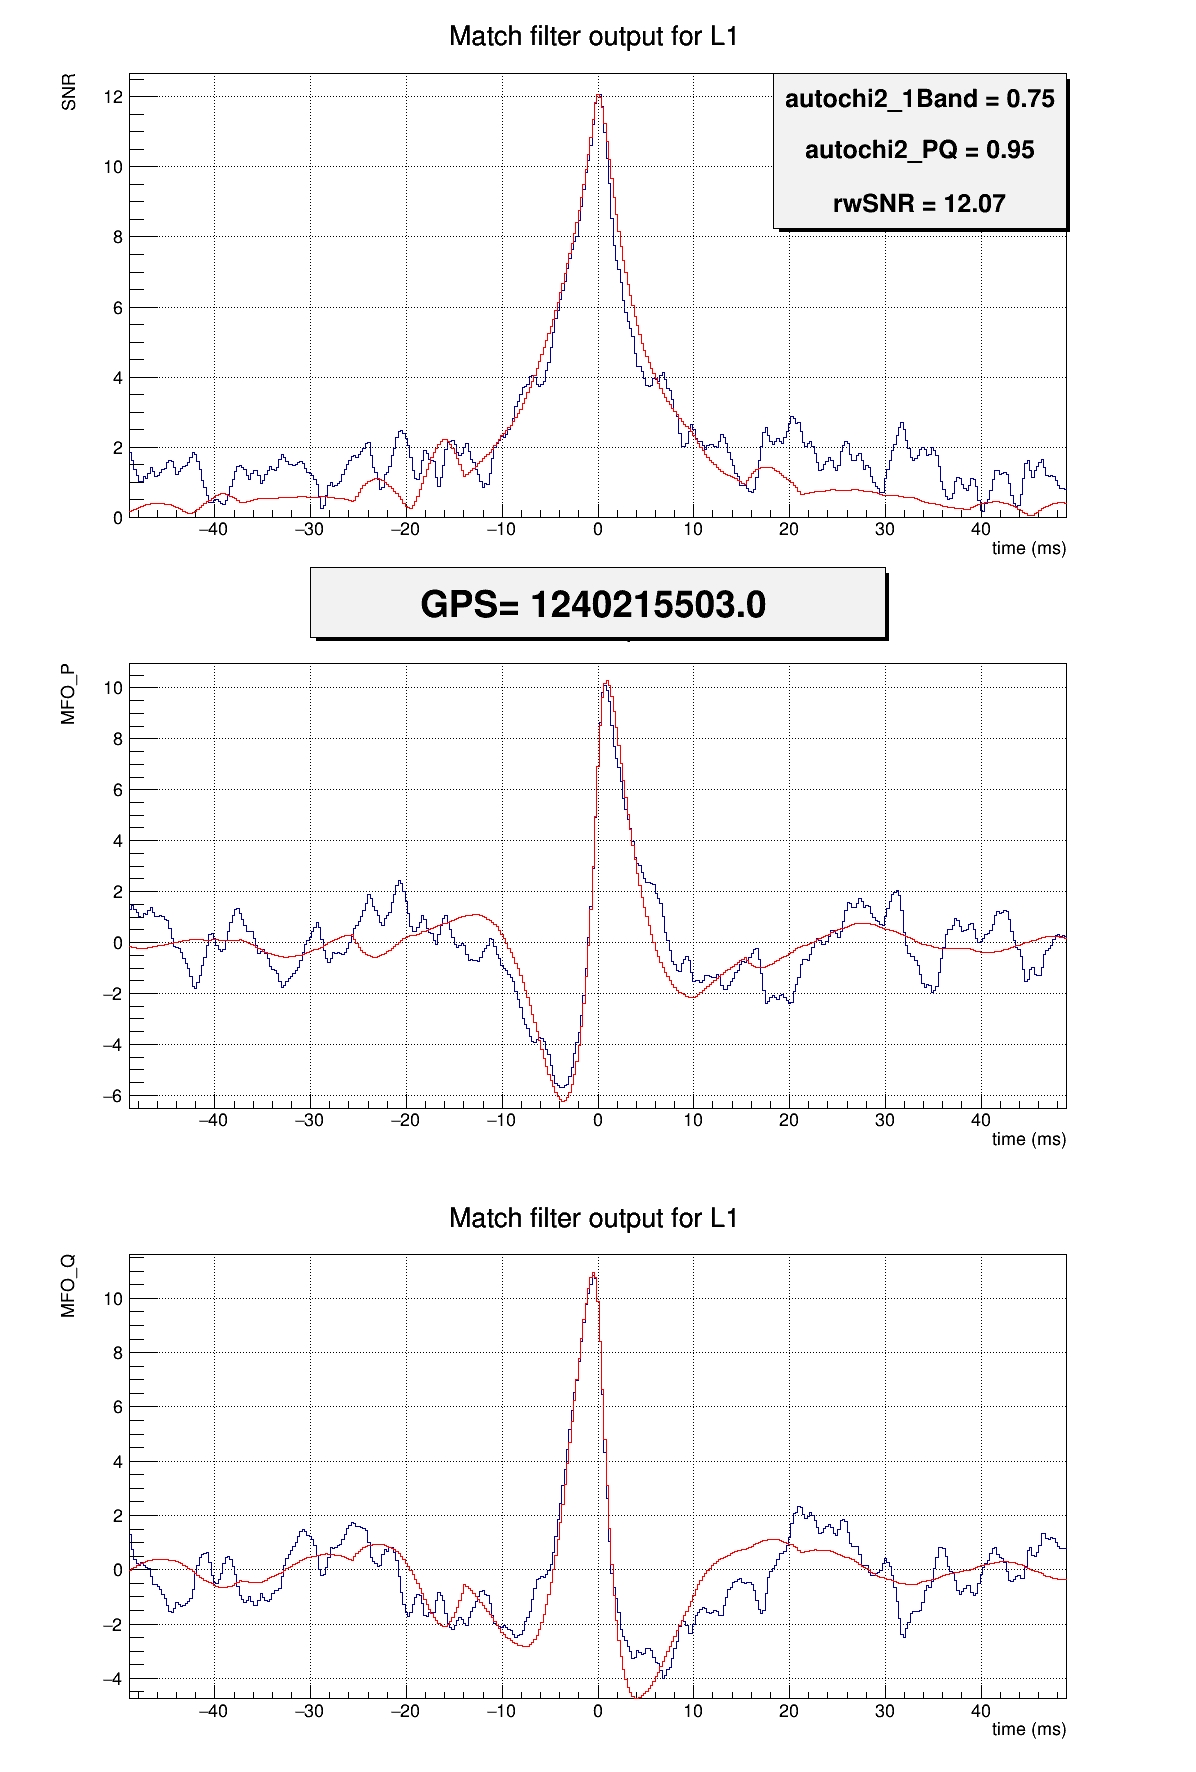
\includegraphics[width=\linewidth]{sectionMBTA/mfoAstro.png}
  \end{minipage}
  \hfill
  %
  \begin{minipage}{0.45\linewidth}
    \centering
    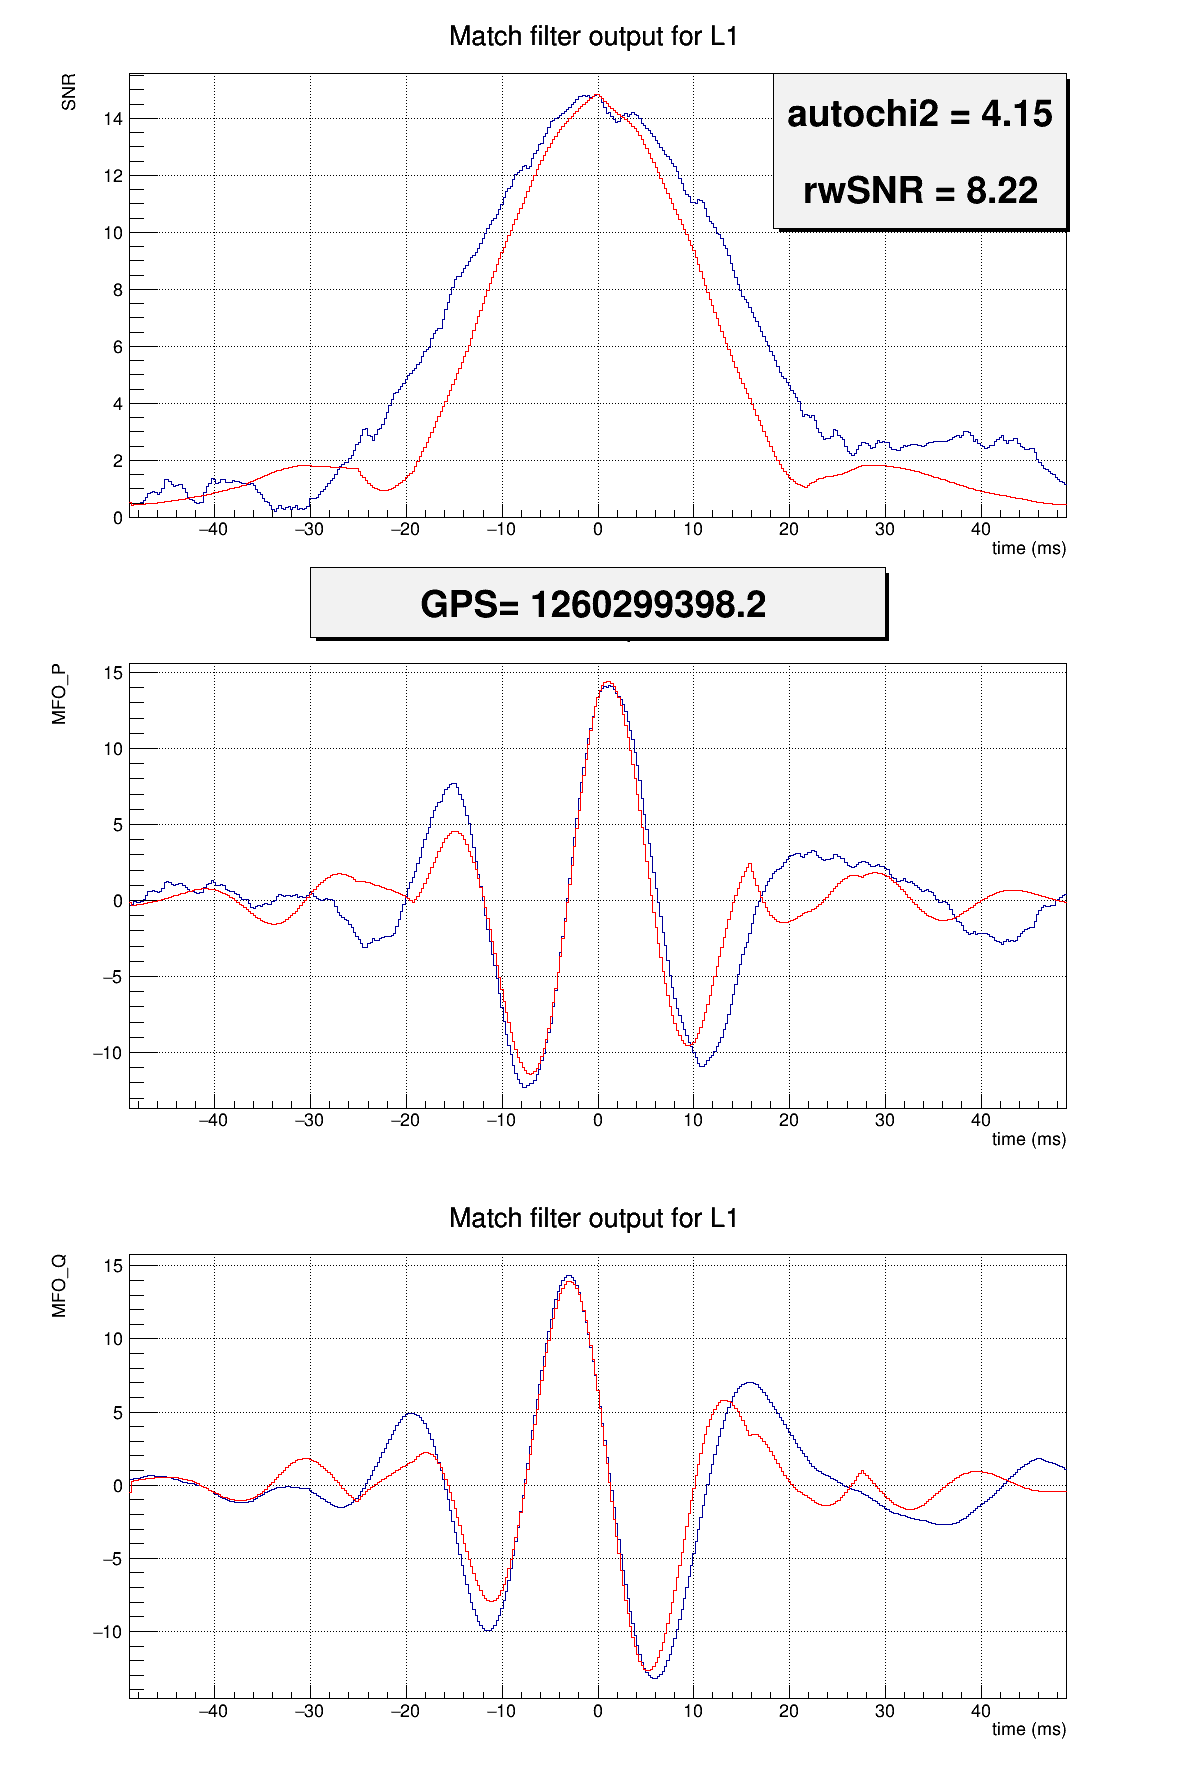
\includegraphics[width=\linewidth]{sectionMBTA/mfoGlitch.png}
  \end{minipage}
  \caption{Left: Measured (blue) and expected (red) MFOs for astrophysical event GW190425 in L1. Right: Measured (blue) and expected (red) MFOs for a loud noise event.}
  \label{fig:mfo_achi2}
\end{figure}
%

Further considerations on the \achi are given in chapter \ref{sec:improve_achi2}.


\subsubsection{Excess rate and ranking statistics}
\label{sec:er}
The excess rate is computed from the trigger rates before and after applying the rwSNR: let $r_{raw}$ be the raw rate of triggers (i.e. above the SNR threshold with only the gating applied) and $r_{sel}$ the rate of triggers above the rwSNR threshold, the excess rate at time $t_0$ is
%
\begin{equation}
\label{eq:ER}
    \textrm{ER}(t_0) = \underset{t_0-10s \leq t \leq t_0}{\textrm{median}}\left( \frac{r_{raw}(t) - r_{sel}(t)}{r_{raw}(t)} \right)
\end{equation}
%

It is then used to reweight again the SNR \textbf{after the coincidence step} (see section \ref{sec:coinc_search}) and yield the ranking statistics (RS):
%
\begin{equation}
\label{eq:rank_stat}
  \textrm{rank stat} = \begin{cases}
    \textrm{rwSNR}, & \textrm{if ER $\leq 0.3$}.\\
    \textrm{rwSNR} \times \left[1-A(\textrm{ER}-0.3)^\alpha \right], & \text{otherwise}.
  \end{cases}
\end{equation}
%
with $\text{A}=1$, $\alpha = 2$.



\subsection{Coincidence search}
\label{sec:coinc_search}
We expect astrophysical events to produce correlated signals across detectors in terms of arrival time, phase and amplitude.
It is much more likely for an astrophysical signal to be found in several detectors than for a glitch or noise fluctuations due to non-stationarity.
Considering coincidences therefore excludes many noise triggers from the analysis.
Thus, to ensure more significant and reliable detections as well as to better probe low SNR events, coincidences between the different detectors are searched for.
Events found in coincidences between detectors also have the benefit to provide a much better estimation of the source location as explained in section \ref{sec:network}.
Finally a threshold is applied on the ranking statstic of coincidences to keep only the most significant events.

Triggers found in different detectors must satisfy two conditions to be considered as coincident:
%
\begin{itemize}
\item the time delay between them must be smaller than a given threshold to take into account the time of flight of the GW from one detector to the other,
  typically \SI{15}{\milli\second} for H1-L1 and \SI{35}{\milli\second} for H1-V1 and L1-V1;
\item their template parameters must match exactly (i.e. same template).
\end{itemize}
%

A coincidence between two (three) detectors is called a double (triple) coincidence.
They are denoted by the initial letters of the interferometers that participated in the coincidence.
For example a coincidence between LIGO Livingston and Virgo is an LV coincidence, a triple is written HLV.
Coincidences are first constructed as doubles and if an HL and HV share a common H1 trigger they are upgraded to an HLV coincidence.
During triple detector time, a double coincidence can be significant enough to be uploaded to GraceDB.
In this case we also search for a subthreshold trigger in the third detector.
If one is found the event is upgraded to a pseudo-triple coincidence and, if for instance the third detector is Virgo, it is named HL-Von. .
Pseudo-triple coincidences uploaded to GraceDB have the combined SNR and skymap computed using the information of the three detectors but their significance is kept as the one of the double.
This is done in order to provide a better sky localization of the source.

The SNR$^2$ of a coincidence is taken as the quadratic sum of the SNR of the single detector triggers, for example
%
\begin{equation}
  \rho_{HL} = \sqrt{\rho^2_{H1} + \rho^2_{L1}}
\end{equation}
%
Contrary to the combined SNR of the triple coincidence, its combined ranking Statistic (cRS) is not simply the quadratic sum of the single detector triggers ranking statistics.
This is motivated by the fact that for an astrophysical source, the signal observed across the different detectors is expected to have some correlation from one detector to another.
The quantities expected to show some correlation are namely the arrival time of the signal, the phase of the signal and its amplitude.
For any two detectors $a$, $b$ the combined ranking statistic is given by
%
\begin{equation}
  \rho^2_{RS,ab} = \rho^2_{RS,a} + \rho^2_{RS,b} + 2\ln\left(P_{\Delta t_{ab}} P_{\Delta \Phi_{ab}} P_{\Delta RA_{ab}}\right)
  \label{eq:CRS_double}
\end{equation}
%
with the probabilities $P_{\Delta t_{ab}}$, $P_{\Delta \Phi_{ab}}$, $P_{\Delta RA_{ab}}$ respectively for the time of flight, phase difference and relative amplitude and $\rho^2_{RS,a}$ as given by eq. \ref{eq:rank_stat}.

The combined ranking statistic for a triple coincidence (with detectors labeled $a$, $b$, $c$) is then derived as
%
\begin{equation}
  \rho^2_{RS,HLV} = \rho^2_{RS,HL} + \rho^2_{RS,HV} - \rho^2_{RS,H}
  \label{eq:CRS_triple}
\end{equation}
%
where we avoid counting twice the RS of H1 since triple coincidences are built from HL and HV triggers.

The probabilities in eq. \ref{eq:CRS_double} are called parameter consistency tests.
They are derived from distributions of simulated BNS with chirp mass \SI{1.2}{\msun}, no spin and uniformely distributed in a sphere of radius \SI{300}{Mpc}.
Since these parameters are derived from the source location, we expect the same behaviour for all type of sources at first order (the timing resolution for heavy BBH compared to BNS is neglected).
Not all of these injections can actually be detected because some are too distant.
An injection is detectable by a detector if its effective distance is within the horizon of this detector.
We consider here horizons of \SI{100}{Mpc}, \SI{140}{Mpc} and \SI{50}{Mpc} for H1, L1 and V1 respectively.
The distribution of the parameters for the injections detectable as double coincidences (triples included) are shown in figure \ref{fig:pct_inj_selec}.
Note that we are only selecting on the generated parameters of the injections, no MBTA analysis is done here.

The similarity in sensitivity and antenna pattern between the two LIGO detectors make the HL distribution rather simple.
The phase difference between H1 and L1 follows a distribution centered on $\pi$.
The mean distance ratio between the two is slightly less than one, as expected due to their range difference.
Large time differences are deprecated because they would require a source located on the line passing by the two detectors which constitutes a small part of the sky.
It is therefore less likely to have such detections.

Regarding the two LIGOs and Virgo, the overlap between their different antenna patterns make things more complicated.
Their antenna pattern are rotated by $\sim 45°$ causing more detection with phase difference closer to $\pi/2$ and $3\pi/2$.
The mean distance ratio is larger than one in favour of H1 and L1, owing to the differences in ranges.
The time of flight distributions are roughly uniform and also depend on the orientation of the detectors.

The correction applied to the cRS are derived from these distribution after including a model of the detector resolution for these parameters.
More details can be found in \cite{aubin2020}.
We show in figure \ref{fig:pct_correc} the corrections applied to the cRS$^2$ as a function of the various parameters for each pair of detector.

Finally we show in figure \ref{fig:pct_inj_recov} the distributions of the same parameters for O3 common injections recovered by MBTA.
We can see that their shape is very close to the ones described previously.

% \begin{figure}
%   \centering
%   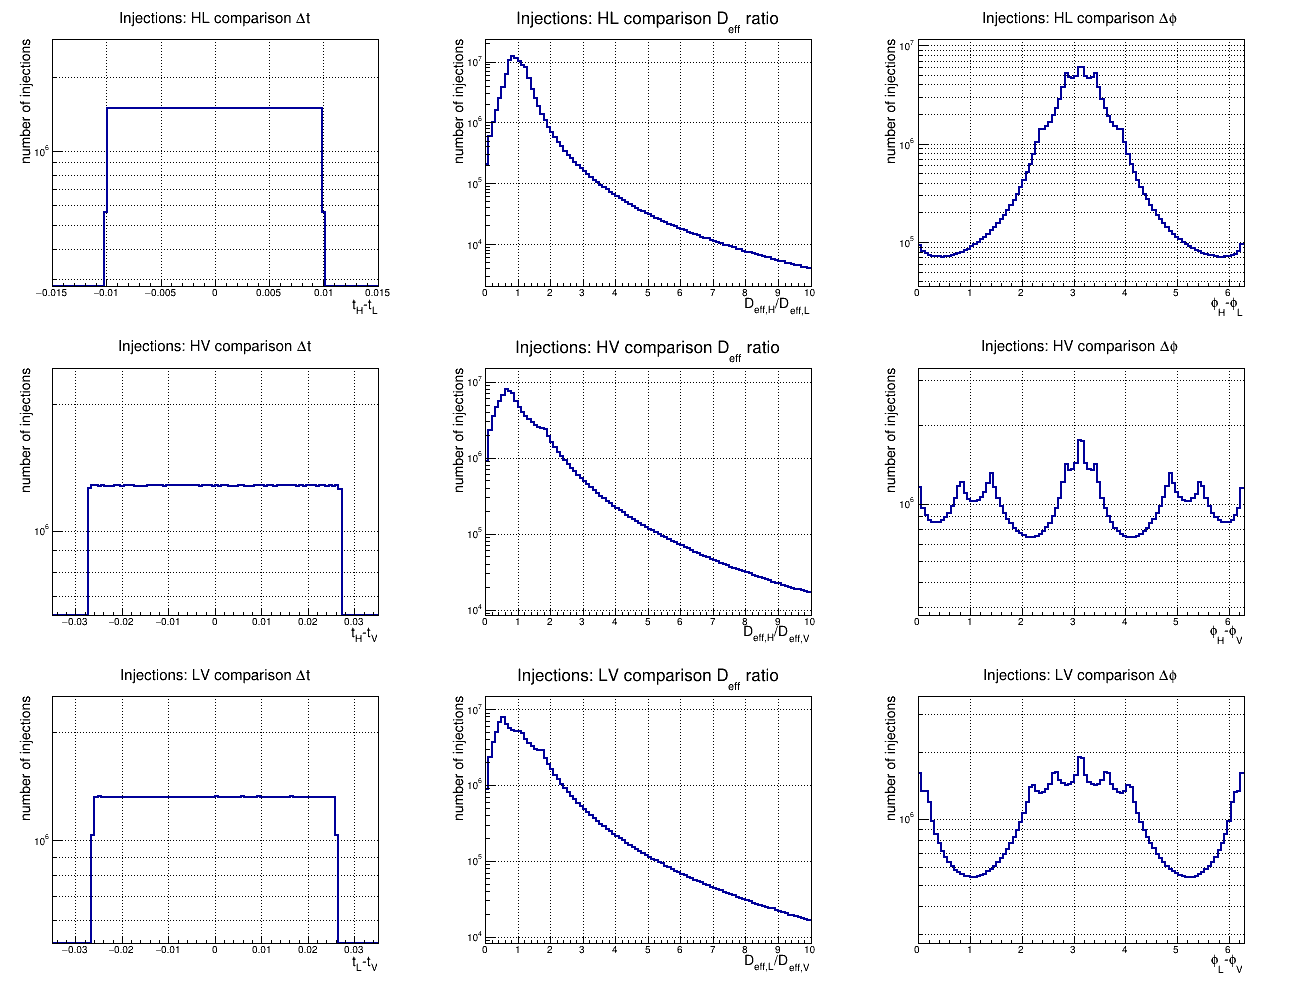
\includegraphics[width=\linewidth]{sectionMBTA/cInj.png}
%   \caption{Comparison of the parameters of the injections.\textcolor{red}{retirer}}
%   \label{fig:pct_inj}
% \end{figure}

\begin{figure}
  \centering
  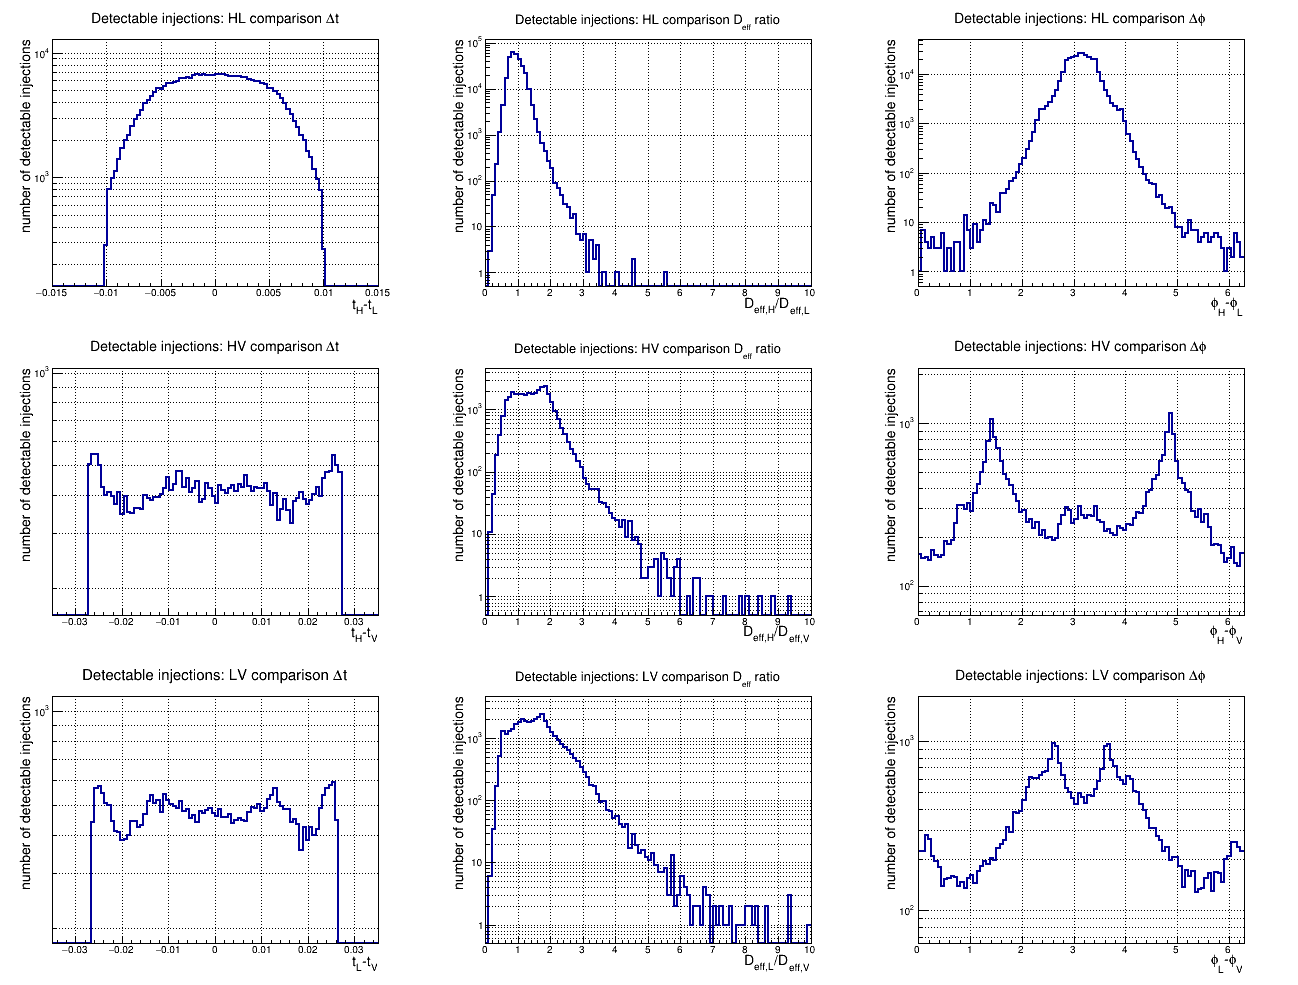
\includegraphics[width=\linewidth]{sectionMBTA/cInjDoub.png}
  \caption{Comparison of the parameters of the injections detectable by at least two detectors.}
  \label{fig:pct_inj_selec}
\end{figure}

\begin{figure}
  \centering
  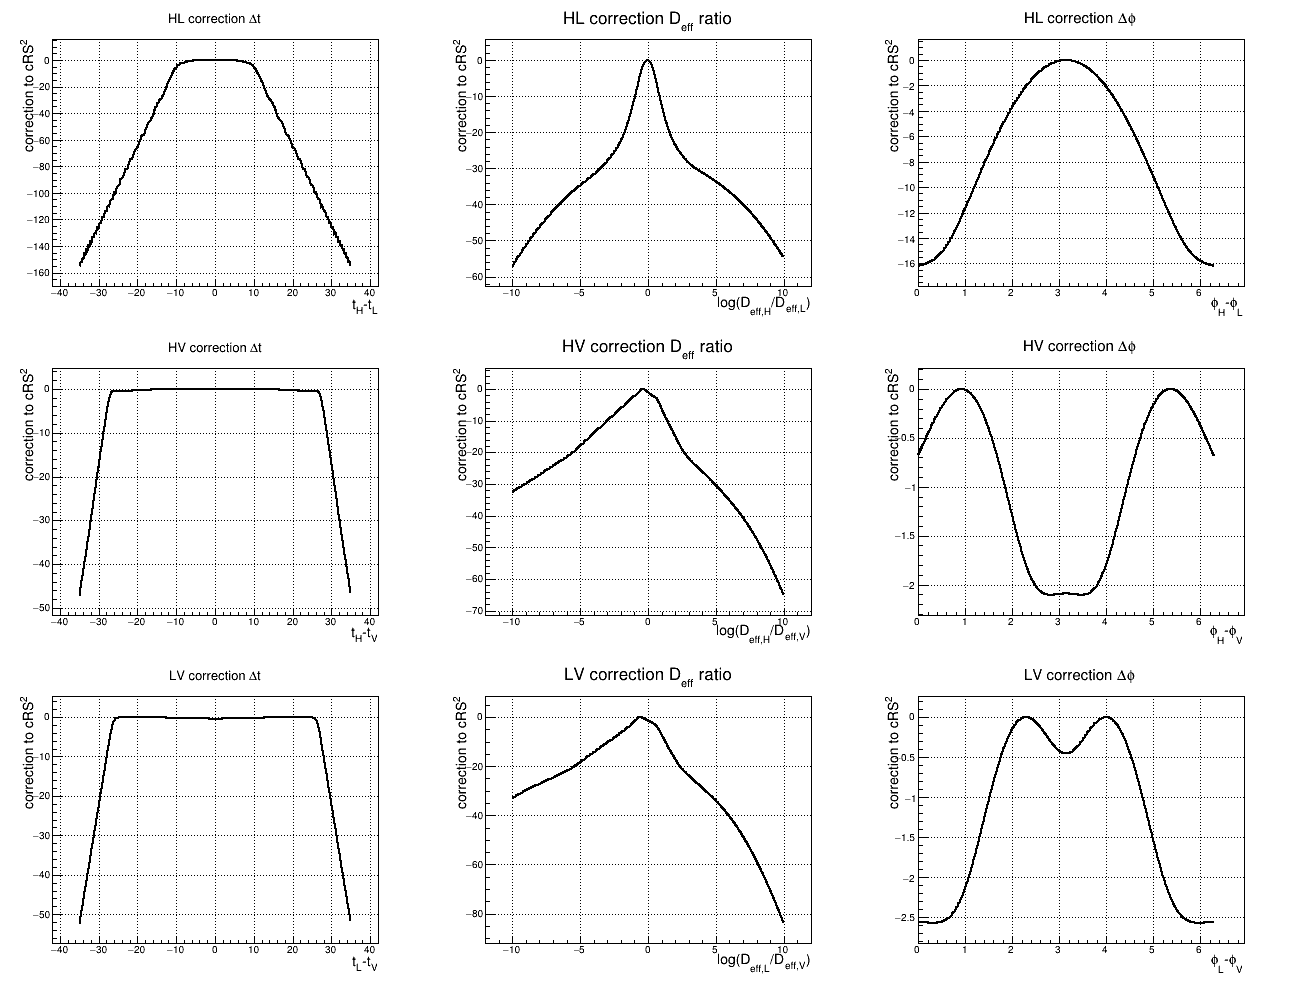
\includegraphics[width=\linewidth]{sectionMBTA/cPCT.png}
  \caption{Correction applied to the cRS$^2$ for each parameter and pair of detector.}
  \label{fig:pct_correc}
\end{figure}

\begin{figure}
  \centering
  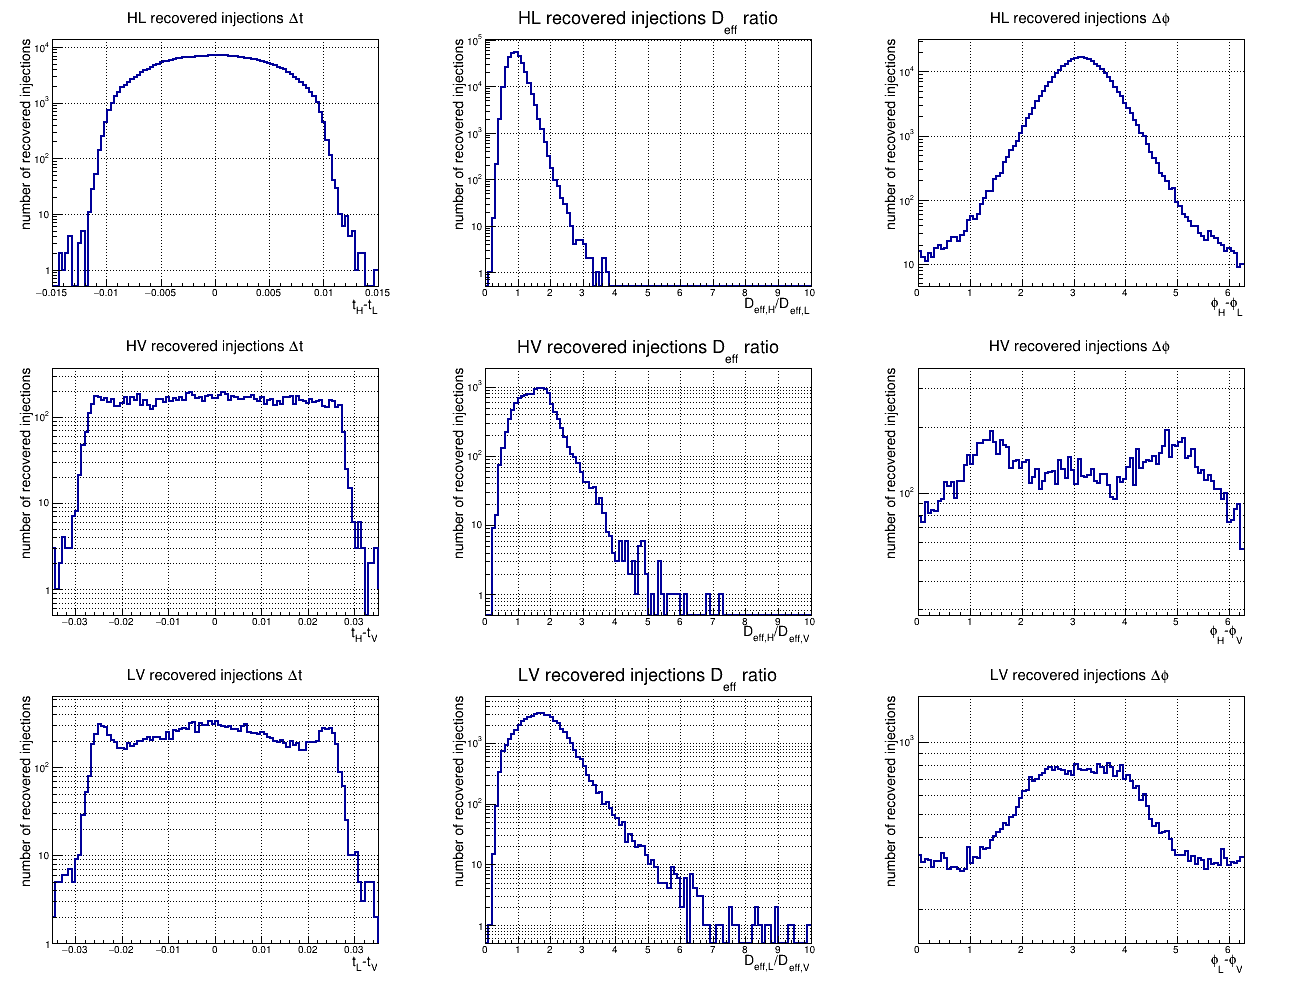
\includegraphics[width=\linewidth]{sectionMBTA/cRecovInj.png}
  \caption{Comparison of the parameters of recovered O3 common injections.}
  \label{fig:pct_inj_recov}
\end{figure}



\subsection{Clustering}
\label{sec:clustering}

A loud astrophysical signal or glitch can match with more than one templates, producing several triggers.
To avoid counting such events multiple times the concept of clustering was introduced in the search.
Clustering consists in merging every trigger within a certain time gap of each other into what is called a clustered event or simply cluster.
This means that triggers apart from more than the time gap can still be part of the same cluster as long as they have a common neighbor within said time gap, as shown by figure \ref{fig:cluster}.
The time gap is typically of $\sim$ \SI{10}{\milli\second}.
The clustered event takes all the parameters (SNR, masses, spins...) of the most significant trigger in the cluster also called ``cluster head''.
MFO vectors of the head are also saved, along a few vectors containing the most relevant parameters of the other triggers of the cluster.
The size of the cluster is characterized by the number of trigger it contains as well as its $t_{\textrm{before}}$ and $t_{\textrm{after}}$, the time differences between the cluster head with the earliest and latest trigger in the cluster respectively.



\begin{figure}[ht]
  \centering
  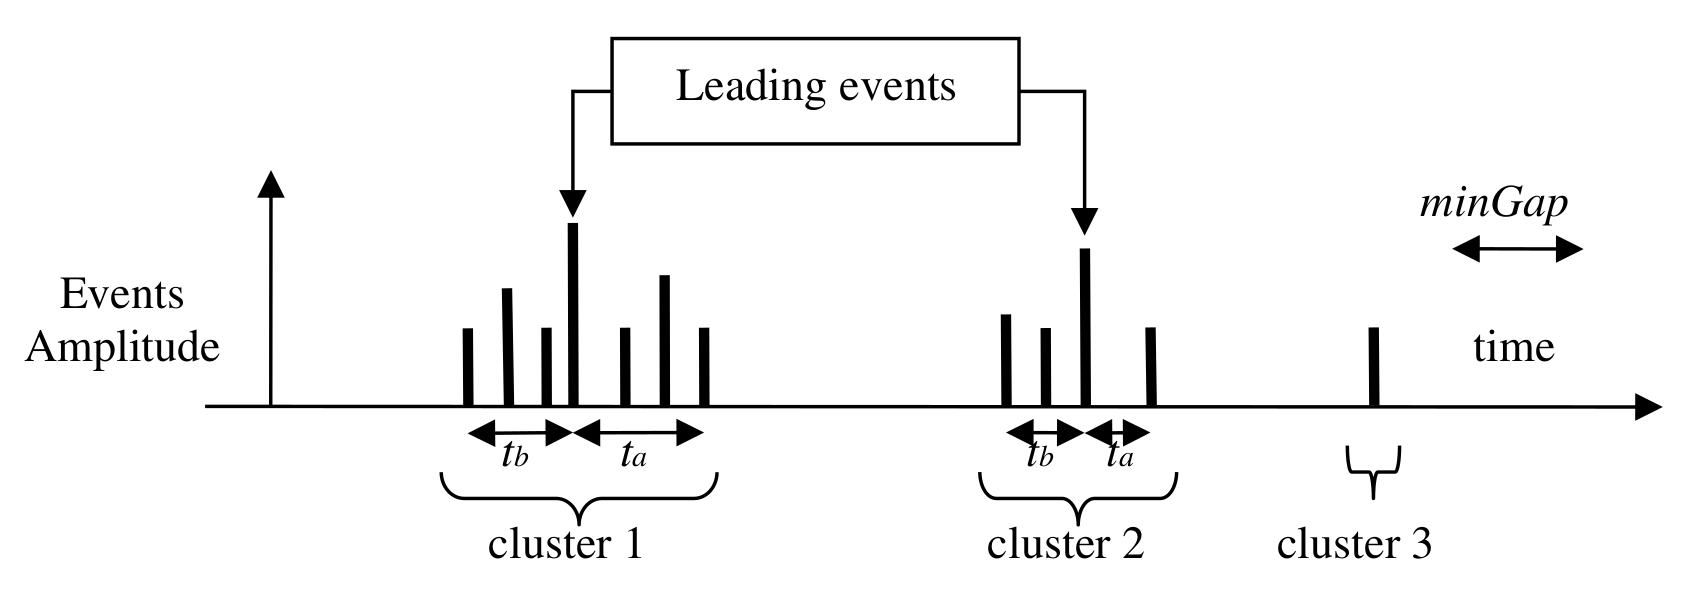
\includegraphics[width=\textwidth]{sectionMBTA/clustering.png}
  \caption{Scheme for the clustering process taken from MBTA's documentation. Vertical bars represent events and are proportional to their SNR, $t_b$ and $t_a$ correspond to $t_{\textrm{before}}$ and $t_{\textrm{after}}$ respectively. In the case of cluster 3, which contains only one event, $t_{\textrm{before}} = t_{\textrm{after}} = 0$.}
  \label{fig:cluster}
\end{figure}




%%%%%%%%%%
\subsection{FAR computation during O3}
\label{sec:far_coinc}
\subsubsection{FAR for a single search}

In the following paragraphs we will refer to a given region of the O3 parameter space and a given type of coincidence as an individual search.

The false alarm rate (FAR) indicates how likely it is for a background trigger to have a given cRS.
It is computed as the rate of background triggers expected above a given cRS threshold.
Upon detection of a candidate with combined ranking statistics $\rho_{RS,0}$ we need to know what this expected rate is.
To this end we compute a cRS distribution for background triggers which straightforwardly gives a FAR vs cRS distribution.

The background distribution used in the computation of the FAR for an individual search is built by making random coincidences between the two relevant detector's single detector triggers.
Times where astrophysical signals have been identified are excluded.
Due to the very high number of low SNR events they are down-sampled to reduce the computational cost.
During O3 the online analysis collected single detector triggers in such a way over the last 24 hours for each search region, while the offline analysis used $\sim$ 6 days.
The background distribution for the coincidences is then built by combining any single detector triggers with matching templates, independently of their arrival time.
The large number of fake coincidences is expected to smooth large noise fluctuations or correlations that might have occured in the detectors.
The CRS of the fake coincidences is computed using the single detector triggers parameters for the phase and amplitude and a random time of flight value (within the range permitted for the two considered detectors).

A FAR is first computed for each individual search and then a final FAR is computed by taking into account the different searches and the time covered by at least two properly working detectors.
This is motivated for instance by the fact that a double coincidence during triple detector time is not the same as a double coincidence during double detector time, we have less information for the latter.

The FAR for a given CRS threshold is then given by
%
\begin{equation}
  \textrm{FAR}_{ab}(\rho_{RS,ab}) = N_{ab}(\rho_{RS,ab}) \frac{\omega_{ab}}{T_a T_b}
  \label{eq:FAR_double}
\end{equation}
%
where $N_{ab}(\rho_{RS,ab})$ is the number of fake coincidences with CRS equal or larger than the threshold $\rho_{RS,ab}$, $\omega_{ab}$ is the coincidence time window and $T_a$ and $T_b$ are the analyzed times for detector $a$ and $b$.

In the case of a triple coincidence, since they are built for HL and HV coincidences, we can compute their FAR from the FAR of the doubles.
This is done by integrating the product of the FAR of the HL and HV coincidence while being careful not to count twice the triggers in H1 .
We then need to renormalize it by the triple detector time $T_{HLV}$ and by the number of triggers in H1 $N_H(\rho_{RS,H})$:
%
\begin{equation}
  \textrm{FAR}_{HLV} = \int\int \frac{ \textrm{FAR}_{HL}(\rho_{RS,HL}) \textrm{FAR}_{HV}(\rho_{RS,HV}) }{N_H(\rho_{RS,H})/T_{HLV}} d\rho_{RS,HL}d\rho_{RS,HV}
  \label{eq:FAR_triple}
\end{equation}
%
with $\rho^2_{RS,H} = \rho^2_{RS,HL} + \rho^2_{RS,HV} - \rho^2_{RS,HLV}$ (eq. \ref{eq:CRS_triple}).
All of this allows to compute the FAR for the $3 \times 4 = 12$ individual searches.
Figure \ref{fig:far_crs} shows a typical FAR vs cRS distribution obtained by making fake coincidences with single detector triggers.

\begin{figure}[ht]
  \centering
  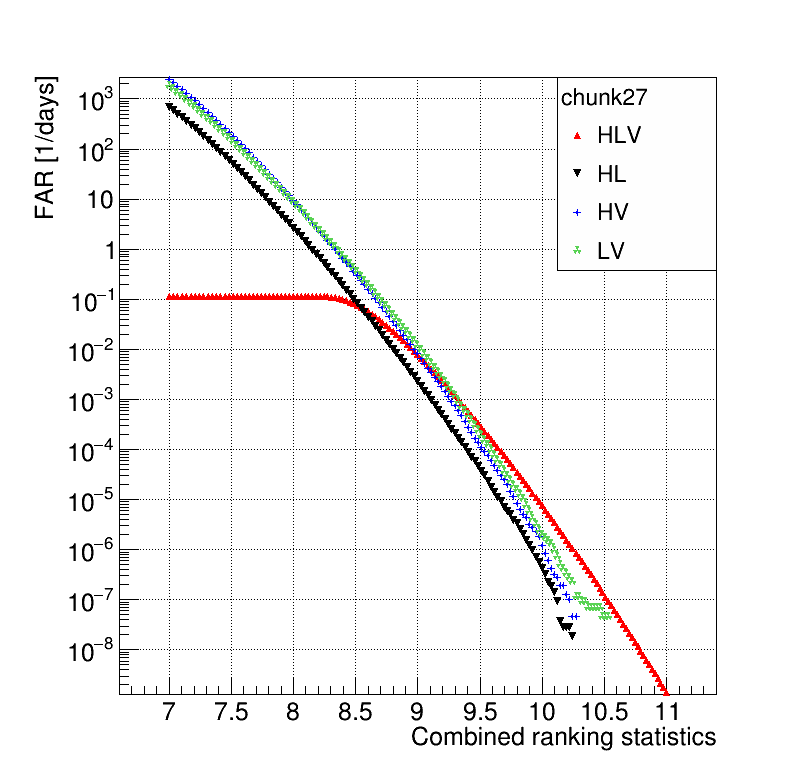
\includegraphics[width=0.5\linewidth]{BNSFARcRank_chunk27.png}
  \caption{Double and triple coincidences FAR vs cRS distribution obtained by combining single detector triggers of the O3 BNS (region 1) search from December 3 2019 to December 11 2019. Clustering and trial factors are not applied yet.}
  \label{fig:far_crs}
\end{figure}

The background is computed using unclustered triggers, but the clustering reduces the overall number of triggers which would lead to inconsistent IFAR cumulative distributions.
To take this effect into account the FAR is scaled by a factor $k_{\textrm{cluster}}$ which is the average ratio of the number of clustered events versus the number of events before clustering.
For the O3 online analysis we had $k_{\textrm{cluster}} = 0.59$ for the BNS region and $k_{\textrm{cluster}} = 0.44$ for the BBH and NSBH regions.
The Inverse False Alarm Rate (IFAR) of a coincidence from a given individual search is given by
%
\begin{equation}
  \textrm{IFAR} = \frac{1}{k_{\textrm{cluster}} \textrm{FAR}(\rho_{RS})}
\end{equation}
%


\subsubsection{Global search FAR}
By construction each of the background distributions computed for the individual searches yields the same rate of noise coincidences with FAR below a given threshold.
This means that we could take a straightforward approach and simply weight each of the 12 distribution before combining them into a single one.
This was done by putting the same weight $k_{\textrm{region}} = 1/3$ on the three search regions, which favours the BNS region because of its astrophysical interest despite its reduced number of templates.
For the type of coincidences, however, some astrophysical priors were included to improve the search:
First, not all coincidences are equivalent in the sense that they are not as likely to seize astrophysical signals.
The distributions are scaled by a trial factor $k_{\textrm{coinc}}$ to take into account the relative difference in search volume of the different type of coincidences.
This search volume is estimated through an injection run (see later section \ref{sec:inj}) by counting the number of injections recovered by the different type of coincidences.
During O3 triple detector times we had $k_{\textrm{coinc}} = 0.909$, $0.002$, $0.007$ and $0.083$ for HL, HV, LV and HLV respectively.
For double detector time it was first set to 1 for the online analysis and later set to the fraction of double-detector volume versus triple-detector volume for the offline analysis.
Figure \ref{fig:ifar_cum} shows the IFAR cumulative plot for double and triple coincidences during a few days (same period as figure \ref{fig:far_crs}) of O3 where no astrophysical signals were detected.


\begin{figure}[ht]
  \centering
  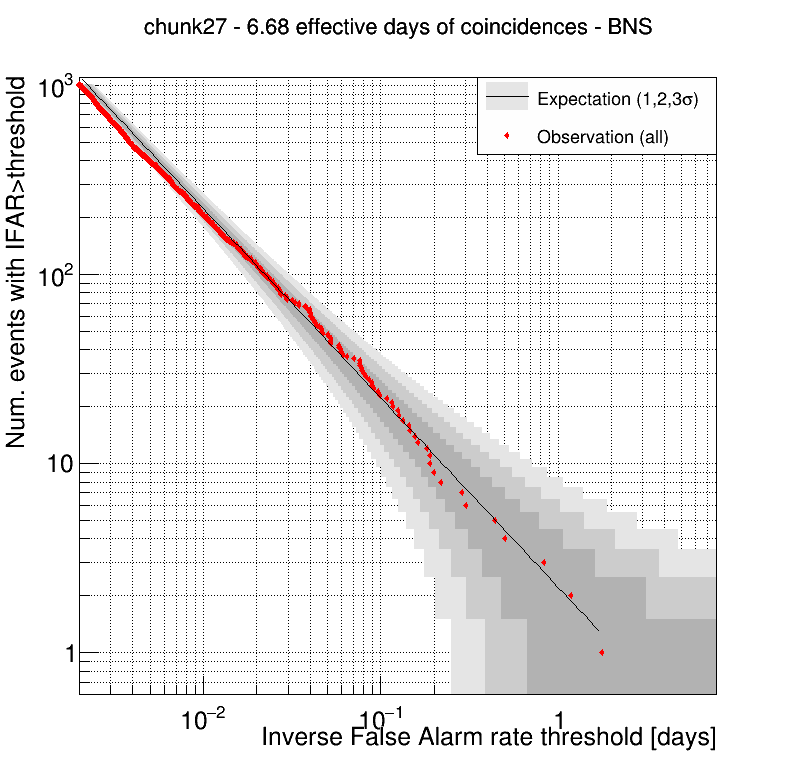
\includegraphics[width=0.5\linewidth]{sectionMBTA/IFAR_cum_chunk27.png}
  \caption{IFAR cumulative plot for double and triple coincidences during 6.68 effective days for the O3 BNS (region 1) search. The observation is consistent with expectations for background only.}
  \label{fig:ifar_cum}
\end{figure}







%%%%%%%%%%
\subsection{Probability of astrophysical origin and source classification}
\label{sec:pastro}

The increasing number of GW detections allows to have more information on the source populations.
The knowledge of these populations can be used to compute a probability of astrophysical origin when a candidate is detected.
This probability is complementary to the FAR.
It will help detecting more astrophysical signals in regions of the parameter space that are denser in sources.

In addition to the probability of astrophysical origin, source populations can be used to infer a source classification of the candidates.
Being able to classify the sources allows to compute merger rates for the different type of sources.

Both the probability of astrophysical origin and the source classification are helpful to astronomer during low-latency searches to decide whether to follow-up on the alert.
The methods to compute them for MBTA were developped during the offline analysis of O3.

More recently, methods to compute the probability of having a neutron star and a probability of having a remnant mass after merger were developped for MBTA in preparation for O4.

\subsubsection{p$_{\textrm{astro}}$, p$_{\textrm{source}}$}
With the insight gained on the source populations, thanks to all the detections made, it is possible to infer a probability of astrophysical origin as well as developp a source classification for the candidates we detect.
The method used by MBTA, fully described in \cite{pastro}, is the following.
The probability of astrophysical origin is computed as
%
\begin{equation}
  p_{\textrm{astro}} = \frac{\textrm{astrophysical foreground rate}}{\textrm{astrophysical foreground rate} + \textrm{background rate}}
\end{equation}
%
Assuming a normalized foreground and background distribution in cRS$^2$, $f($cRS$^2)$ and $b($cRS$^2)$ respectively, for a given observing time where we expect $N_f$ foreground triggers and $N_b$ background triggers we have
%
\begin{equation}
  p_{\textrm{astro}} = \frac{N_f f(\textrm{cRS}^2)}{N_f f(\textrm{cRS}^2) + N_b b(\textrm{cRS}^2)}
\end{equation}
%
The source (BNS, BBH, NSBH) classification is derived from this expression as
%
\begin{equation}
  p_{\textrm{source}} = \frac{N_{\textrm{source}} f_{\textrm{source}}(\textrm{cRS}^2)}{N_f f(\textrm{cRS}^2) + N_b b(\textrm{cRS}^2)}
\end{equation}
%
with
%
\begin{equation}
  p_{\textrm{BNS}} + p_{\textrm{BBH}} + p_{\textrm{NSBH}} = p_{\textrm{astro}}
\end{equation}
%
In practice the expected rates of astrophysical and background candidates are not a priori known and need to be estimated from the data.
This is done by assuming the foreground and background as independent Poisson processes and using Bayes' theorem to compute the posterior distribution of counts assuming a distribution of cRS$^2$.
Since we do not expect the same type and rate of astrophysical events in all regions of the parameter space, the latter is divided in bins of chirp mass and mass ratio for a total of 165 bins during O3.
Each bin has its own foreground and background distribution.
One last thing that needs to be taken into account is that the different types of coincidences (doubles, doubles in triple detector time, triples) will have different astrophysical foreground rates because of the detector sensitivities and orientations.
This is accounted for by weighting the foreground for each type of coincidence, the weight being computed using injections.

\subsubsection{hasNS, hasRemnant}
As was previously discussed, one of the motivation for gravitational waves detection is to participate in multi-messenger searches.
Since we can now provide a source classification, it would be interesting to be able to tell if a signal is likely to have an electromagnetic counterpart.
We call such events ``EM bright''.
A definition of the EM bright population for the pipeline MBTA will be given in section \ref{sec:embright}.
For that we define two quantities: hasNS and hasRemnant.
The first one is the probability that the binary system had a neutron star, the latter is the probability that there is some matter remaining after the merger (with mass above a given threshold).
The definition for hasNS is rather straightforward:
%
\begin{equation}
  \textrm{hasNS} = \frac{p_{\textrm{BNS}} + p_{\textrm{NSBH}}}{p_{\textrm{astro}}}
\end{equation}
%
For hasRemnant it gets more complicated because not all NSBH mergers have a remnant mass.
We define hasRemnant as
%
\begin{equation}
  \textrm{hasRemnant} = \frac{p_{\textrm{BNS}} + p_{\textrm{NSBH-bright}}}{p_{\textrm{astro}}}
\end{equation}
%
To define what is a bright NSBH we make two assumptions:
\begin{itemize}
\item BNS mergers have a remnant mass, meaning $p_{\textrm{BNS}}=1 \Rightarrow \textrm{hasNS}=\textrm{hasRemnant}=1$,
\item BBH mergers have no remnant mass, meaning $p_{\textrm{BBH}}=1 \Rightarrow \textrm{hasNS}=\textrm{hasRemnant}=0$.
\end{itemize}
We need to tell whether a NSBH will have a remnant mass.
Foucart et al. \cite{remnant} have given a parametrization for the remnant mass after the merger of a neutron star and black hole with masses $M_{\textrm{BH}}$ and $M_{\textrm{NS}}$ respectively:
%
\begin{equation}
  M^{\textrm{rem}} = M^b_{\textrm{NS}} \left[ \textrm{Max}\left( \alpha \frac{1-2C_{\textrm{NS}}}{\eta^{1/3}} -\beta \frac{R_{\textrm{ISCO}}}{M_{\textrm{BH}}} \frac{C_{\textrm{NS}}}{\eta} + \gamma, 0 \right) \right]^\delta
\end{equation}
%
where $M^b_{\textrm{NS}}$ is the baryonic mass of the neutron star, $C_{\textrm{NS}}$ its compactness (neutron star mass over neutron star radius in natural units), $\eta$ the symmetric mass ratio $q/(1+q)^2$ and $R_{\textrm{ISCO}}$ the radius of the innermost stable circular orbit.
The baryon mass is related to the neutron star mass by the binding energy
%
\begin{equation}
  \textrm{BE} = M^b_{\textrm{NS}} - M_{\textrm{NS}}
\end{equation}
%
which is in turn related to the compactness of the star \cite{binding_energy} by
%
\begin{equation}
  \frac{\textrm{BE}}{M_{\textrm{NS}}} = d_1 C_{\textrm{NS}} + d_2 C_{\textrm{NS}}^2
\end{equation}
%
Since the compactness directly depends on the neutron star equation of state, and since this latter is not too constrained (as presented in section \ref{sec:EOS}), a marginalization over the mass-radius EOS posterior given in \cite{Legred_2021} is carried out.
A NSBH is considered bright if the predicted remnant mass is larger than \SI{1.e-3}{\msun}.


\subsubsection{Evolution for O4: FAR(p$_{\textrm{astro}}$)}
\label{sec:far_coinc_O4}

When making catalogs of detected events during O3, some issues were raised regarding the consistency between FAR and p$_{\textrm{astro}}$.
Indeed, for a same value of p$_{\textrm{astro}}$, there were some large differences in FAR.
This can be explained by the fact that, during O3, the FAR was computed on the 3 regions of the parameter space while p$_{\textrm{astro}}$ was computed on 165 bins:
the astrophysical foreground can vary greatly (several orders of magnitude) from one bin to the other but the background changes by at most an order of magnitude.

To solve these issues, it was decided to use another method for O4.
A FAR based on the cRS tells how likely it is for background to produce a loud event.
This is definitely good and was especially usefull when we had little knowledge on the signals we detect.
We now have more knowledge and we use it to tell how likely it is for a trigger to be an astrophysical signal through the computation of p$_{\textrm{astro}}$.
The question that we ask now is: how likely is it for a background event to have a given p$_{\textrm{astro}}$ value.
To answer this question we decide to compute a FAR of p$_{\textrm{astro}}$, meaning that p$_{\textrm{astro}}$ will play the role previously fullfilled by the cRS$^2$.
We have on one side FAR$($cRS$^2)$ and on the other p$_{\textrm{astro}}($cRS$^2)$ which can be inverted and combined to give a FAR$($cRS$^2($p$_{\textrm{astro}}))$ which is computed for each type of coincidence, each type of network configuration (number of detector online) and each p$_{\textrm{astro}}$ bin.
This FAR is then summed over all bins and integrated over the observing times corresponding to the network configurations available for each type of coincidence (i.e. over single, double and triple detector time for single detector triggers, double and triple detector time for double coincidences and triple detector time for triple coincidences).


